\lhead{\begin{tikzpicture}[remember picture, overlay]
    \node [anchor=100,inner sep=0] (imagenIZQUIERDA) at (current page header area.north){
\includegraphics[width=18cm]{img/Encabezado.PNG}};
    \end{tikzpicture}}
    \rhead{Piedra-Moreno}
    \rfoot{\begin{tikzpicture}[remember picture, overlay]
    \node [anchor=140,inner sep=0] (imagenDERECHA) at (current page footer area.south){
\includegraphics[width=18cm]{img/Foot.PNG}};
    \end{tikzpicture}}
    %----------------------------------------------------------------------------------------
    \lfoot{ \thepage}
    % \renewcommand{\labelenumi}{\alph{enumi}.)} 
    %----------------------------------------------------------------------------------------
    %----------------------------------------------------------------------------------------
    %	TITLE SECTION
    %----------------------------------------------------------------------------------------
    
    \setlength{\droptitle}{-5\baselineskip} % Move the title up
    \title{\textbf{Estudio de tiempos y movimientos en el ensamble de un circuito electrónico utilizando diferentes métodos para su optimización }} % Article title
    
     \author{ 
     \textsc{Piedra-Moreno, Alitza Alejandra}\\ 
     \texttt{ Instituto Tecnológico de Querétaro } \\ 
     \texttt{ Tecnológico Nacional de México } \\ 
     \texttt{Querétaro, México}\\ 
     \texttt{l22140912@queretaro.tecnm.mx} 
     \and 
     \textsc{Ángeles-Hurtado, Luis Alberto}\\ 
    %  Afiliación:
     \texttt{ Instituto Tecnológico de Querétaro } \\ 
     \texttt{ Tecnológico Nacional de México } \\ 
     \texttt{Querétaro, México}\\ 
     \texttt{alb3rt0.ah@gmail.com} 
    }
    
    
    %----------------------------------------------------------------------------------------
    
    % \begin{document}
    
    % Print the title
    \maketitle
    \thispagestyle{fancy}
    
    %----------------------------------------------------------------------------------------
    %	ARTICLE CONTENTS
    %----------------------------------------------------------------------------------------
    
    % \section*{Resumen}
    % \textit{Palabras clave:}
    % El resumen (ancho de página) deberá contener entre 100 y 200 palabras tipo Adobe Devangari 11 puntos.
    
    \begin{abstract}
    \noindent 
    El resumen (ancho de página) deberá contener entre 100 y 200 palabras tipo Adobe Devangari 11 puntos.
    
    \end{abstract}
    % 
    % 
    \textbf{\textit{Palabras clave}}: {Estudio, análisis, tiempo, movimiento, estándar, empresa, industrial, operación, muestra}
    % \keywords{First keyword should be the corresponding to the research area according with the authors guide. Maximum of 6 keywords.}
    
    \section{Introducción}
    
    La mejora de un proceso representa un reto para las industrias, ´ estas invierten una cantidad importante de capital con ese fin. El destino de esos recursos se orienta a la compra de nueva maquinaria, a la capacitación del personal, y al esfuerzo por alcanzar estándares de calidad más competitivos. Sin embargo, destinan poco dinero al desarrollo de tecnología.\cite{83520408}
    
    En el contexto industrial, un ensamblaje se refiere al proceso de unir o conectar múltiples componentes individuales para formar un producto final o una parte de un producto más grande. Este proceso implica la unión de piezas mediante diversos métodos. El ensamblaje electrónico se refiere al proceso de unir y conectar componentes electrónicos individuales para formar un sistema electrónico funcional. Este proceso es fundamental en la fabricación de una amplia variedad de dispositivos electrónicos, desde teléfonos inteligentes y computadoras hasta dispositivos médicos y sistemas de control industrial.
    
    Así mismo, los circuitos electrónicos son componentes fundamentales en la industria moderna, permitiendo la automatización, el control, la eficiencia energética, el monitoreo en tiempo real, la calidad del producto, la innovación y la seguridad laboral. Su importancia es tal que sin ellos, muchas operaciones industriales serían difíciles, costosas o simplemente imposibles de realizar. En sí, el ensamble de un circuito electrónico es un proceso complejo que involucra múltiples etapas, desde la selección y adquisición de componentes hasta la soldadura y pruebas finales. Para optimizar este proceso, se pueden emplear diversos métodos y estrategias, dentro de los cuales se encuentran el estudio de movimientos y tiempos, el estudio de tiempos predeterminados, el muestreo del trabajo, balanceo de líneas, datos estándar y entre otros.
    
    El estudio de movimientos y tiempos, está definido como el análisis de los movimientos, herramientas, materiales, e instalaciones utilizadas y que se han de utilizar, teniendo como meta encontrar la forma más económica de realizar el trabajo, normalizar los métodos, materiales, herramientas e instalaciones, determinar el tiempo estándar y ayudar al aprendizaje de los métodos. Con esto en mente podemos inferir que su objetivo es la optimización, que significa buscar las herramientas para que el proceso se ejecute en el mejor tiempo posible, que ofrezca mejores resultados y que economice, o de forma más simple, obtener los mejores resultados posibles de manera eficaz y eficiente  \cite{RAE}. En la actualidad las empresas u organizaciones, sin importar su tamaño e industria, enfrentan enormes desafíos que les exigen ser competitivas en el mercado globalizado, la productividad de las empresas se ve más afectada por la distribución y relaciones de las plantas, entre diferentes sectores empresariales. Las empresas buscan la mejor manera de integrar herramientas basadas en estudios de métodos y medición de procesos utilizando observación directa y secuencial de procesos, determinando diagramas de flujo, tiempos, distancias, actividades, funciones, tiempos de inactividad, expectativas, almacenamiento, transporte, aquí se toman referencias para comparar, decidir e implementar cambios y tendencias para aumentar la eficiencia de la producción. 
    
    Un método es el estudio de movimientos, que es el análisis cuidadoso de cada uno de los movimientos que se emplean para realizar una tarea o de otra parte identificar cada uno de los Therbligs utilizados, lo cuales se comprenden como los 17 movimientos básicos divididos en eficientes e ineficientes. \cite{niebel1980ingenieria} En este análisis se tiene como objetivo eliminar los innecesarios para obtener una mayor eficiencia, incluyendo la comprensión del factor humano, así como el conocimiento, las materiales herramientas e instalaciones.
    
    Por otra parte, el sistema de tiempos predeterminados, está definido como el conjunto de reglas o principios con el fin de determinar y resolver con anticipación la secuencia de pasos o sucesos.\cite{RAE}. Cabe mencionar que los STP tienen como base el uso de los Therbligs, y a estos elementos le asignan a cada uno un valor de tiempo, por otra parte, se incursiona la medición de distancias y métodos con el fin de sacar un estándar, por esto mismo podemos decir que su desventaja es que son automáticos y depende de los juicios del analista por ende no siempre son exactamente precisos.
    
    Como otro método para la optimización del ensamblaje, tenemos el muestreo del trabajo el cual consiste en generar un método de muestreo, donde se escogerá las muestras más representativas que sean de calidad, que describan de manera exacta las características de un conjunto de un fenómeno, que nos permitan predecir, deducir, inferir y sacar conclusiones de este ensamble, y lograr ser lo más exacto y preciso posible, además nos sirve para disminuir los costos que presenta un estudio continuo del tiempo o estudio de tiempos convencional, el cual implica un esfuerzo y trabajo mayor, y lo más importante un mayor costo económico. Para este método que se implementara se deberá utilizar mucho las probabilidades y estadísticas, con el fin de tener una precisión más exacta y que nuestros datos sean los más parecidos a los reales.
    
    Así mismo con el motivo de generar una precisión más exacta se utilizará el tiempo productivo el cual es la calificación del desempeño del operador, basándonos en la experiencia, capacitación, y juicio del analista, esto con motivo de normalizar y estabilizar los tiempos generando un intervalo de tiempos menor, reduciendo así el intervalo de confianza. Con esto en mente tenemos el objetivo de realizar estas muestras, para poder deducir lo que es el tiempo ciclo y estándar a través de lo que es la probabilidad y estadística con la cual nos centraremos en o que es el método del límite central para generar una media que nos ayudara a ser más exactos en el tiempo estándar de nuestra operación, ayudándonos a tener una visión más clara de nuestras bases para posteriormente generar una mejora, en el método, materiales, distribución y hasta instalaciones.
    
    Otro de los métodos que se pueden utilizar es el balanceo de líneas que es una herramienta muy útil para el control de la producción de una industria, dado que una línea de fabricación equilibrada permite la optimización de variables que afectan la productividad de un proceso tales como: inventarios de productos en proceso, los tiempos de fabricación y las entregas parciales de producción. El objetivo principal por el cual se realiza un balanceo de línea corresponde a la igualación de los tiempos de trabajo en todas las estaciones del proceso y el incremento de la eficiencia en general.\cite{‌Euroinnova}
    
    
    
    En contraparte, los estándares de trabajo que se calculan a partir de los datos y fórmulas estándar son relativamente consistentes, ya que los elementos calculados son el resultado de muchos estudios de tiempos probados con cronómetro. Como los valores están tabulados, solo es necesario sumar los elementos que se requieren para establecer un estándar, y todos los analistas deben llegar a estándares de desempeño idénticos para un método dado. Por lo tanto, se asegura la consistencia de los estándares establecidos por diferentes analistas en una planta, al igual que de los distintos estándares calculados por un determinado observador de estudio de tiempos. Por lo general, los estándares de un trabajo nuevo pueden calcularse con mayor rapidez mediante los datos o fórmulas estándar que a través de un estudio de tiempos con cronómetro. \cite{‌23}
    
    
    
    En la actualidad, cuando hablamos de datos estándar, nos referimos a todos los estándares de elementos tabulados, gráficas, nomogramas y tablas que permiten medir una tarea específica sin el empleo de un dispositivo medidor del tiempo, como un cronómetro. Los datos estándar pueden tener varios niveles de refinamiento: movimiento, elemento y tarea. Mientras más refinado sea el elemento del dato estándar, más amplio será su rango de uso. Por lo tanto, los datos estándar de movimiento tienen la mayor aplicación, pero toma más tiempo desarrollarlos que cualquier dato estándar de una tarea o un elemento. Una fórmula del estudio de tiempos es una presentación alternativa y, típicamente, más sencilla del dato estándar, en especial en el caso de los elementos variables. Las fórmulas tienen aplicaciones específicas en el trabajo no repetitivo, para el cual no es práctico establecer estándares para cada tarea con un estudio de tiempos individual. La construcción de una fórmula implica el diseño de una expresión algebraica que establece un tiempo estándar antes de la producción, sustituyendo valores conocidos propios de la tarea para los elementos variables.\cite{‌23}
    
    Actualmente, el sector de la fabricación ha experimentado avances importantes en la integración de inteligencia artificial para la mejora de un sinfín de operaciones. En este GRID de IA  hemos recogido el pulso de un buen número de organizaciones que trabajan en la integración de esta tecnología en los procesos de producción.
    
    En su mayoría, las voces de la industria proclaman la llegada de la IA a los dinámicos sistemas de producción como una fuerza impulsora clave que redefine los límites de la automatización y la robótica industrial. A medida que avanzamos hacia este futuro cercano, varios aspectos destacados de la IA están preparados para desempeñar un papel fundamental en la optimización y mejora de los procesos industriales. \cite{rouhiainen2018inteligencia}
    
    Como otro método que se puede utilizar tenemos la optimización industrial que toma el modelado y la simulación de procesos, como una herramienta fundamental para el estudio o análisis gráfico, físico o matemático de los procedimientos y actividades de un sistema de producción de una organización, con el fin de crear un nuevo diseño digital que automatice, optimice y logre la eficacia y la eficiencia de los procesos, suprimiendo errores y anticipando soluciones que alcancen en plenitud los objetivos de dicha organización.
    
    La simulación de procesos industriales permite esquematizar los procesos generando modelos virtuales donde se pueden identificar los errores, verificando el layout, anticipándose a los resultados de los procesos de producción de manera precisa y sin correr riesgos.
    
    Con el modelado y la simulación de procesos industriales podemos optimizar los tiempos de los procesos, examinando diferentes alternativas. Además, obtenemos la facultad de analizar las fases críticas de procesos como la ergonomía, la producción, el mantenimiento, la logística, la layout (disposición de medios), entre otros; acentuando la calidad y la precisión del diseño. Igualmente, se obtiene la supresión de costos extra, ya que se puede verificar, revisar y automatizar el diseño de optimización en tiempo real. \cite{sanchez2015analisis}
    
    Con todo esto en mente, resumimos que a través de todos estos métodos y teniendo en cuenta los avances en la industria para la optimización de los ensambles así como los métodos antiguos, los que se busca encontrar en este artículo es el diseño, mejora e integración de sistemas productivos aplicando todas etas tecnologías para una dicha optimización, mediante la mejora continua, el análisis y estandarización.
    
    
    \section{Justificación}
    
    La industria constituye la actividad más importante de la producción material en la mayoría de los países. Tal y como se conoce hoy, esta actividad se desarrolla a partir de la revolución industrial en Inglaterra y ha estado estrechamente ligada al progreso en los países capitalistas más avanzados.
    
    Durante la mayor parte de la centuria pasada, los economistas llegaron a establecer una conexión directa entre industrialización y desarrollo, fundamentalmente sobre la base de la experiencia de los países ricos y, luego, de la extinta Unión de Repúblicas Socialistas Soviéticas (URSS). Varios economistas destacados, como Rosenstein-Rodan (1943), Prebisch (1950), Lewis (1954), Hirschman (1958) y otros, le otorgaron un lugar central a la manufactura en el esfuerzo de desarrollo de los países más atrasados. Su valor se relacionó con la explotación de economías de escala junto a una alta y creciente productividad del trabajo; su papel, con la mejoría de los términos de intercambio, el acelerado cambio técnico y una gran capacidad de impactar en el avance de otras ramas a través de encadenamientos productivos. Kaldor (1966), por ejemplo, resaltó que estos elementos permitían explicar la presencia de rendimientos crecientes, lo que estaría detrás del colapso del crecimiento económico en estados industrializados que experimentaran una pérdida sostenida de su tejido industrial. 
    
    
    
    La mayoría de estos efectos se han manifestado claramente en la trayectoria de un grupo de nuevos países industrializados (NPI), esencialmente en Asia, pero también en el caso de Irlanda y Brasil. Un aspecto especialmente relevante tiene que ver con su impacto en el avance científico-técnico y en la innovación-desarrollo (I+D). Datos recientes (McKinsey Global Institute MGI, 2012) indican que más del 90 \% del gasto en I+D en el sector productivo se origina en la manufactura; mientras que las cinco revoluciones tecnológicas descritas hasta la actualidad (Pérez, 2002) han tenido como punto de partida la actividad industrial, para luego generar considerables externalidades hacia el conjunto del sistema económico.
    
    Estas consideraciones forman parte de la agenda de desarrollo para las naciones pobres y, por supuesto, también para Cuba. Por ello es indispensable conocer las tendencias más importantes del desarrollo industrial en el mundo y sus consecuencias para la formulación de políticas en este grupo de estados
    
        En la actualidad, la competitividad de las empresas es considerada una cuestión fundamental en los sectores económicos tanto de los países desarrollados como en desarrollo. El contexto internacional y en especial el proceso de globalización requieren que las organizaciones cuenten con recursos eficaces y eficientes en la gestión de los recursos financieros, humanos, naturales y tecnológicos, entre otros, para afrontar el desafío del mercado, no solo nacional, sino fuera de las fronteras de sus países de origen. \cite{labarca2007consideraciones}
        
        En el nivel medio o marco, la competitividad está relacionada con las ventajas relativas de los recursos de un país o región, ya sea tierra, trabajo y capital, o con las ventajas que surgen principalmente de las inversiones en formación de capital humano e innovación. \cite{padilla2006instrumento}
        
        En la situación actual, donde prevalecen continuos y rápidos cambios tecnológicos, la formación juega un papel muy importante para fortalecer la competitividad de la empresa, como productora de capital humano. Por un lado, complementa la formación formal, proporcionando al empleado los conocimientos y habilidades necesarios para utilizar, adaptar y, en última instancia, mejorar la tecnología. Por otro lado, dado que tiene como objetivo proporcionar a los empleados los conocimientos y habilidades que necesitan en sus operaciones diarias, se puede esperar que genere un retorno rápido y significativo para la empresa.\cite{casar1993competitividad}
        
        Desde comienzos de año, diversos indicadores muestran una clara divergencia entre la actividad del sector manufacturero y el sector servicios. De hecho, según los índices PMI globales, la actividad manufacturera se está enfriando desde inicios del pasado año (y se encuentra ya estancada o en retroceso en algunos países), mientras que el sector servicios ha mostrado una notable recuperación.
        
        Parte de esta divergencia entre manufacturas y servicios responde a su diferente naturaleza cíclica. El consumo de bienes duraderos y la producción manufacturera son muy cíclicos y sensibles a cambios en las condiciones monetarias. Por tanto, es lógico pensar que la notable tensión experimentada por las condiciones monetarias globales desde comienzos de 2022 ha terminado enfriando la actividad en el sector industrial. Sin embargo, existen otros motivos que explican que la discrepancia sectorial actual se encuentre en máximos desde la crisis financiera de 2008. \cite{CaixaBank}
        
        Querétaro es uno de los estados con el mayor número de parques industriales del país, donde están asentadas empresas mexicanas, estadounidenses, alemanas, canadienses y coreanas.
        
        El sector industrial en el estado de Querétaro, aporta el 36 por ciento de los empleos totales en la entidad. Es decir, hay 352 mil puestos laborales en este sector. Esto debido a que se tiene un total de 49 parques industriales en la entidad.
        
        Querétaro se ha destacado a lo largo de los años por su notable crecimiento económico y por mantenerse en los primeros lugares dentro de los indicadores de actividad económica. Este significativo desarrollo económico e industrial se refleja en que Querétaro es de los estados con mayor número de parques industriales del país. \cite{JessicaIgnot}
        
        En el estado se tiene registro de 67 parques y zonas industriales, que se concentran principalmente en El Marqués (34.3\%), Querétaro (31.1\%), Colón (13.4\%); los restantes están en Pedro Escobedo, Huimilpan, Corregidora y Cadereyta (20.9\%), expone el Anuario Económico Estatal, edición 2021, de la Secretaría de Desarrollo Sustentable.
    
    % 
    % 
    \section{Descripción del problema}
    
    El problema de optimización del ensamble electrónico es multifacético y requiere un enfoque integral que tenga en cuenta la eficiencia, los costos, la calidad, la flexibilidad y la tecnología. Al utilizar varios métodos y enfoques, las empresas pueden mejorar la eficiencia y la competitividad de sus operaciones de ensamble electrónico en un mercado cada vez más exigente.
    
    Otro de los problemas que encontramos en este estudio es que al utilizar el método de muestreo, se reducirán los costos, pero el problema será encontrar una muestra que sea representativa de la población, así como encontrar el valor esperado real y la variación de nuestros datos.
    
    Otro de los problemas que nos hemos de encontrar será el sacar el tiempo ciclo así como el buen análisis de tiempo productivo además que al usar el método de sistemas de tiempos predeterminados el juicio del analista sea el correcto, ya que este puede variar entre analista y no suele ser el más preciso y exacto.
    
    Por otra parte, una de nuestras incógnitas científicas es el tiempo ciclo, que es el que en nuestro estudio es el primer elemento a sacar para el inicio de nuestro análisis. Así mismo describimos el problema como la baja productividad y eficiencia que contenemos en nuestro ensamblaje, por ello mesmo debemos buscar un método en el cual nuestro circuito eléctrico pase de un elemento inestable con el movimiento, difícil de identificar las partes, costoso y desordenado a un elemento de fácil manejo, identificación simple de los elementos, simpleza de los pasos para los empleados y un costo menor, el cual será un gran beneficio para la empresa. 
    
    También contamos con la incógnita de sí el método probabilístico será el correcto, ya que al final solo son suposiciones, por lo que se espera que el valor obtenido sea el más cercano, mientras que nuestros datos sean los correctos.
    
    \section{Fundamentación teórica}
    
    Los términos estudio de tiempos y estudio de movimientos fue creado por W. Taylor y Frank B. Gilbert y su esposa Lilian M. El estudio de movimientos y tiempos implica el análisis de movimientos, herramientas, materiales e instalaciones utilizadas y que se han de utilizar y consta de 4 etapas:
    \begin{enumerate}
        \item Encontrar la forma más económica de hacer el trabajo.
        \item Normalizar los métodos, materiales, herramientas e instalaciones usadas.
        \item Determinar exactamente el tiempo necesario para que una persona completamente capacitada realice el trabajo con una marcha normal.
    \item Ayudar al aprendizaje del operario en el método nuevo.
    \end{enumerate}
    
    Por otra parte, el estudio de movimientos implica el análisis cuidadoso de cada uno de los movimientos corporales que se emplean para realizar una tarea, con el fin de eliminar los necesarios para obtener la máxima eficiencia, incluye la comprensión del factor humano así como el conocimiento de los materiales, herramientas e instalaciones. 
    \cite{niebel1980ingenieria}
    
    
    Para esto se debe conocer los movientes básicos, ya que los Gilbreth concluyeron que todo trabajo, ya sea productivo o no, se realiza mediante el uso de combinaciones de 17 movimientos básicos a los que ellos llamaron therblig \cite{niebel1980ingenieria}  
    
    Estos se dividen en eficientes, que estimulan el progreso del trabajo y con frecuencia pueden ser acortados, pero por lo general no pueden ser eliminados:
    \begin{enumerate}
        \item \textbf{Alcanzar (AL):} “Mover” la mano vacía hacia o desde el objeto; donde el tiempo depende de la distancia recorrida.
        \item \textbf{Mover (M):} “Mover” la mano cargada; el tiempo depende de la distancia, el peso y el tipo de movimiento.
        \item \textbf{Tomar (T):} “Cerrar” los dedos alrededor de un objeto, este comienza cuando los dedos tocan el objeto y termina cuando se ha ganado el control.
        \item \textbf{Soltar (SL):} “Soltar” el control de un objeto, normalmente el más corto de los therbligs.
        \item \textbf{Preposicionar (PP):} ”Posicionar” un objeto en una ubicación predeterminada para su uso posterior. Por lo general ocurre en conjunto con “Mover”.
        \item \textbf{Utilizar (U):} “Manipular” Una herramienta para el uso por el que fue diseñada; fácilmente detectable a medida que avanza el progreso del trabajo.
        \item \textbf{Ensamblar (E):} “Unir” dos partes que embonan. Por lo general es precedido por “Posicionar” o “Mover” y seguido por “Liberar”.
        \item \textbf{Desensamblar (DE):} Es lo opuesto a “Ensamblar”, pues separa partes que embonan.
    
     También encontramos los ineficientes, los cuales no representan un avance en el proceso del trabajo y debe eliminarse. En esta categoría encontraremos:
    
        \item \textbf{Buscar (B):} Ojos o manos buscan un objeto; comienza a medida que los ojos se mueven para localizar un objeto.
        \item \textbf{Seleccionar (SE):} “Mover” la mano cargada; el tiempo depende de la distancia. Por lo general es seguido por “Buscar”.
        \item \textbf{Sostener (SO):} Una mano soporta el objeto mientras la otra realiza trabajo útil.
        \item \textbf{Posicionar (P):} “Orientar” un objeto durante el trabajo, por lo general precedido por “Mover” y seguido por “liberar”.
        \item \textbf{Inspeccionar (I):} “Comparar” un objeto con el estándar, típicamente a la vista, pero podría ser también con los demás sentidos.
        \item \textbf{Planear (PL):} “Pausar” para determinar la acción siguiente; por lo general se le detecta como un titubeo que precede a “Mover”
        \item \textbf{Retraso Inevitable (DI):} Más allá del control de quien opera debido a la naturaleza de la operación.
        \item \textbf{Retraso Evitable (DEV):} Quien opera es único/a responsable del tiempo ocio.
        \item \textbf{Descansar (DES):} Aparece periódicamente, no en cada ciclo. Depende de la carga de trabajo física.
    
    \end{enumerate}
    
    De la misma manera se considera el sistema de tiempos predeterminados (STP) los cuales son un conjunto de reglas o métodos para determinar con anticipación la secuencia de sucesos. Este está basado en los anteriormente mencionados Therbligs, ya que a estos elementos les asignaron valores de tiempo, aunque ciertamente los STP “no siempre pueden predecir con precisión” el tiempo que le lleva a un trabajador realizar una tarea. Uno de los problemas de este método es que no son automáticos, es decir, que requiere del juicio del analista. Y esto se menciona, ya que cada analista obtiene tiempos distintos para un mismo trabajo porque interpretan las reglas en forma diversa. Así mismo en los STP lo que mediremos será la distancia, así como los métodos, ya que estos nos ayudaran a estimar él tiempo estándar que nos llevara realizar una tarea. 
    
    
    
    En consiguiente, él métodos de medición del tiempo es un sistema estandarizado para medir los tiempos que tardan los trabajadores en ejecutar una tarea repetitiva. El objetivo de este sistema es analizar donde están los movimientos ineficaces que se traducen en pérdidas innecesarias de tiempo en una tarea que se ejecuta cientos de veces al día. \cite{DanielGrifol}
    
    Cabe resaltar que para hablar de estos métodos debemos describir lo que es la precisión y la exactitud, donde la precisión es lograr la mínima dispersión al momento de hacer una medición o de realizar una tarea. Es la variación o poca variación significa un buen grado de precisión. Y la exactitud se define con respecto a su cercanía o sesgo, mayor cercanía implica un buen grado de exactitud.
    
    Retomando el tema, el muestreo es la acción de escoger muestras representativas de calidad que describa de manera exacta las características de un conjunto que nos dejen deducir, inferir y sacar conclusiones de un fenómeno a estudiar. \cite{RAE} Teniendo en cuanta qué representativo alude a lo significativo, característico, peculiar, relevante e importante. \cite{RAE}
    Por ende, el muestreo de trabajo lo podemos considerar como una herramienta para disminuir el costo que se presenta  en el estudio continuo del tiempo. Su único problema es obtener una muestra representativa. Así mismo utilizando el muestreo del trabajo, reducimos el costo que implica un estudio de tiempos convencional, pero surge el problema de obtener una muestra representativa.
    
    Teniendo en cuenta que el estudio de tiempos convencional, es una muestra continua de n ciclos, suponiendo que la distribución estadística es normal y el estudio de tiempos no convencional contiene huecos entre las lecturas de muestreo y es una muestra discreta suponiendo que la distribución estadística es binomial.
    
    
    Así mismo se utilizará lo conocido como el tiempo productivo, que es la calificación del desempeño de operador, está basada en la experiencia, capacitación y juicio del analista que lo realiza.
    
    
    Con esto en mente en nuestro estudio utilizaremos diversas herramientas como lo es el diagrama de movimientos bimanual la cual es una herramienta que muestra todos los movimientos y retrasos atribuibles a las manos derecha e izquierda, además de la relación que existe entre ellas. Tiene como propósito identificar los patrones de movimiento que resultan ineficientes y observar las violaciones a los principios de la economía de movimientos.\cite{niebel1980ingenieria} Asi mismo, el equipo mínimo requerido para realizar un programa de estudio de tiempos incluye un cronómetro, un tablero de estudio de tiempos, las formas para el estudio y una calculadora de bolsillo. Un equipo de videograbación también puede ser muy útil.
    
    
    En donde en una forma de estudios se registra toda la información pertinente sobre el método que se estudia, las herramientas utilizadas, etc. La operación en estudio se identifica mediante información como nombre y número del operario, descripción y número de la operación, nombre y número de la máquina, herramientas especiales usadas y sus números respectivos, el departamento donde se realiza la operación y las condiciones de trabajo prevalecientes. 
    \cite{niebel1980ingenieria}
    
    Por otra parte, una de las mayores incógnitas que nos surgen será el de cuantos ciclos de estudio deberemos implementar, como el estudio de tiempos es un procedimiento de muestreo, se puede suponer que las observaciones se distribuyen normalmente respecto a una media poblacional desconocida con una varianza desconocida. Si se usa la media muestral y la desviación estándar muestral s, la distribución normal para una muestra grande lleva al siguiente intervalo de confianza \ref{equ:1}. 
    
    \begin{equation}
        \label{equ:1}
        x {\pm} {\frac{zs}{\sqrt{n}}}
    \end{equation}
    
    Pero esto claramente suponiendo que fuera una muestra grande, pero en nuestro caso se entiende que nuestra muestra será menor a 30 por ende se deberá utilizar el método de la T, pero primeramente a falta de tiempo se utilizara el método probabilístico en donde contaremos en el teorema del límite central.
    
    En donde comprendemos al límite central como la exposición y descripción de datos de un fenómeno, y se comprende de verdades admitidas sin demostración, que sirven como base para posteriores razonamientos lógicos y que permiten aproximar magnitudes mediante la secuencia de números, estimando la tendencia central y dispersión de los parámetros. \cite{RAE}
    
    
    \section{Hipótesis}
    Al momento del desarrollo de nuestra optimización, se generarán diversas cuestiones acerca del cómo se debe hacer, cuál es el método adecuado, si lo estamos haciendo correctamente, entre otras. Por ello, se debe prevenir estos problemas con anticipación y generar una hipótesis que nos ayude a trabajar y destacar en los problemas que se deben utilizar.
    
    Al comienzo de nuestro trabajo, tendremos el problema de identificar correctamente las partes de los materiales, pero a medida que avancemos en el desarrollo de la práctica, podremos generar un mayor conocimiento de estos, que nos ayudará a desempeñarnos más en el ensamble y su optimización.
    Otra cuestión, el escaso conocimiento de los métodos de ensamblaje de los circuitos, los cuales, sin duda, existen diferentes, como la impresión 3D, el uso de robots y hasta el uso de inteligencia artificial. Aunque no dispongamos de todas esas tecnologías, tendremos un buen desarrollo de la optimización, ya que contamos con conocimientos recabados y un buen razonamiento.
    
    
    \section{Objetivo}
    
    Diseñar, mejorar e integrar sistemas productivos de bienes aplicando tecnologías para su optimización. Diseñar, implementar y mejorar sistemas de trabajo para evaluar la productividad. Analizar, los movimientos, herramientas, materiales e instalaciones utilizadas y que se han de utilizar para encontrar la forma más económica de hacer, el trabajo. Normalizar los métodos, materiales, herramientas e instalaciones, usadas. Determinar el tiempo necesario y estándar de realización del trabajo.
    
    
    \subsection{Objetivos específicos}
    
    \begin{itemize}
        \item Identificar los materiales, describirlos, recaudar información de ellos, estandarizarlos y normalizarlos.
        \item Crear una secuencia de pasos para estandarizar los procedimientos a realizar en el ensamblaje.
        \item Dividir las operaciones en elementos, para posterior identificar y eliminar los movimientos ineficientes.
        \item Generar un muestro de calidad, y que sea representativo para la toma de tiempos.
        \item Conseguir el tiempo siclo.
        \item Obtener la media muestral y la desviación estándar para estimar lo que es conocido como la media poblacional y la variancia.
        \item Obtener una aproximación al tiempo estándar de la operación.
        
    \end{itemize}
    
    % 
    % \section{Cuerpo }
    
    \section{Cuerpo}
    
    \subsection{Metodología}
    
    Como empresa es importante la mejora continua la cual concite en optimizar, proceso, herramientas e instalaciones, por ello mismo se debe llevar distintos métodos para el desarrollo de esta mejora, pero primero que nada uno como analista debe desglosar y familiarizarse con el método actual, ya que para un buen análisis debemos tener en cuenta todos los factores implicados en el trabajo y además es necesario para una comparativa del antes y él después esto para una mejor aceptación del nuevo método.
    
    Por ello mismo en la figura \ref{fig:Distribucion inicial}se muestra la distribución propuesta para la primera parte del análisis donde aún es con el método actual, lo cual es indispensable para notar los cambias y por ello mismo el operario debe asegurar que esta distribución se cumpla a la hora de realizar la operación.
        \begin{figure}[H] 
        \centering
        \includegraphics[trim = {1mm 1mm 1mm 1mm},clip,scale=0.3]{22/Img/ensamblaje.pdf}
        \caption{Distribución inicial}
        \label{fig:Distribucion inicial}
    \end{figure}
    
    Con esta propuesta de distribución podemos ahora si incursionar al lector a los procedimientos que el operario debe seguir para el desarrollo del ensamble del circuito electrónico, el cual es el método presente o el método propuesto a la mejora y se presenta en la siguiente lista:
    \begin{enumerate}
    
        \item Posiciona el protoboard en el área de ensamblaje.
    
        \item Coloca la ESP32 en el centro del protoboard colocando los pines NC en la columna 30 y en las filas B e I de forma que el pin 3V3 esté en el punto 15-B y quede simétrico, dejando la fila a y j libres. 
    
        \item Conecta un cable MM (azul) en el punto 29-j coincidente al pin G y el otro extremo únelo a la tierra que está del lado de la línea azul (coloca todas las tierras a esta misma línea).
    
        \item Une un cable MM (morado) al punto 15-a, coincidente a 3V3 y conéctalo a la corriente, que es la línea roja (coloca todas las corrientes a esta línea), conecta este cable y la tierra del lado más cercano a la tierra. 
    
        \item Toma el potenciómetro y ensambla el cable amarillo que está soldado al último pin, colócalo en el punto 21-a que es coincidente a la entrada 0.
    
        \item Coloca el cable rojo que está soldado al segundo pin y conéctalo a un cable MM(azul) y este, conéctalo a su vez a la corriente (línea roja), recuerda que se ocupa la misma línea que en el punto 4. 
    
        \item Conecta el cable negro soldado al primer pin del potenciómetro a tierra (línea azul). 
    
        \item Conecta 4 cables MH en la interfaz de la LCD de la siguiente forma, uno blanco en SCL, otro blanco en SDA, un café en VCC y un negro en GND. 
    
        \item El primer cable blanco conéctalo al punto 10-h y en el punto 10-i coloca una resistencia de 330 ohms unida a corriente (línea roja).
    
        \item El segundo cable blanco colócalo en el pin 9-h y de igual forma une una resistencia de 330 ohms al punto 9-i de un lado y del otro a corriente (línea roja).
    
        \item Conecta el cable café directamente a corriente (línea roja) y el negro a tierra (línea azul). 
    
        \item  Conecta un cable MM (naranja) al punto 10-f a lado del cable blanco y del otro lado colócalo en el punto 20-a coincidente con el pin 7
    
        \item Une un cable MM (café) al punto 9-f, junto al otro cable blanco y de la otra punta al punto 19-a en el pin 6 
    
        \item  Enchufa la ESP32 al cable de energía y este cable de energía debe estar conectado a la segunda entrada, la que tiene el botón de BOOT encima.
    
        \item Conecta el multicontacto a la energía y luego conecta el cable de energía a este.
    
    
        \item Asegúrate que la LCD prenda y si ocurre un error oprime el botón RESET colocado en la ESP32
    
    \end{enumerate}
    
    
    Para un mejor desarrollo de la operación, el operario tuvo a su disposición un manual con figuras gráficas, explicando el paso a paso, esta secuencia de pasos a modo de tabla para un mejor entendimiento de este, para observar esta tabla, véase el apéndice \ref{Figura:instructivo}.
    
    \newpage
    \subsection{Materiales}
    
    En el desarrollo de nuestra práctica es indispensable conocer cada una de las partes de nuestro ensamble esto a raíz de que como operario nos es mucho más simple realizar nuestro trabajo si uno conoce y/o se familiariza con cada pieza que se utiliza además que como analista nuestro trabajo es examinar cada parte, medida y hasta material que está implícito en el trabajo para generar una mejora en nuestro método y a su vez implementar el objetivo del estudio del trabajo que es encontrar una forma más económica así como la estandarización de las herramientas, materiales e instalaciones, por ello mismo se debe en listar cada parte del ensamblaje para que a la hora del desarrollo del estudio tengamos una secuencia con orden.
    
    En el apéndice \ref{Figura:Materiales} se muestra cada una de las partes de nuestro ensamble, así como su número de pieza, figura de solidworks y precio.
    
    Con este orden establecido pasaremos a desglosar cada una de las características de nuestras piezas para conocerlas de mejor forma, así como generar  el diagrama y dibujo de cada una de ellas.
    
    \subsubsection{PC-01: Tapete profesional organizador de trabajo, antiestático y magnético}
    
    Una almohadilla de trabajo de reparación electrónica antiestática es una superficie diseñada específicamente para proteger los componentes electrónicos sensibles de daños causados por la electricidad estática. Estas almohadillas están hechas de materiales conductores que disipan la electricidad estática de manera segura, evitando que se acumule en los componentes electrónicos durante el proceso de reparación o montaje.
    
    La almohadilla de trabajo antiestática proporciona una superficie segura y neutral para trabajar con dispositivos electrónicos. Por lo general, tienen una capa superior resistente al calor y a las manchas, proporcionando una superficie de trabajo cómoda y limpia. Además, suelen tener una capa inferior antideslizante para mantenerse en su lugar durante el trabajo.
    
    Es esencial utilizar una almohadilla de trabajo antiestática junto con otras medidas de precaución, como el uso de pulseras antiestáticas o mangas, para garantizar la protección completa de los componentes electrónicos durante la manipulación.
    
    
    E la figura \ref{fig:almohadillaD} se muestra a detalle las medidas de la alfombrilla que se usa como material inicial en el proyecto, esta alfombrilla tuene una superficie de 30x46 cm con tolerancias dimensiónale. Para un mejor trabajo y desempeñó de nuestras operaciones, así como para encontrar una mejora en nuestro método primera mente, se debe conocer el material al 100, por eso mismo el siguiente dibujo.
    
    \begin{figure}[H]
        \centering
        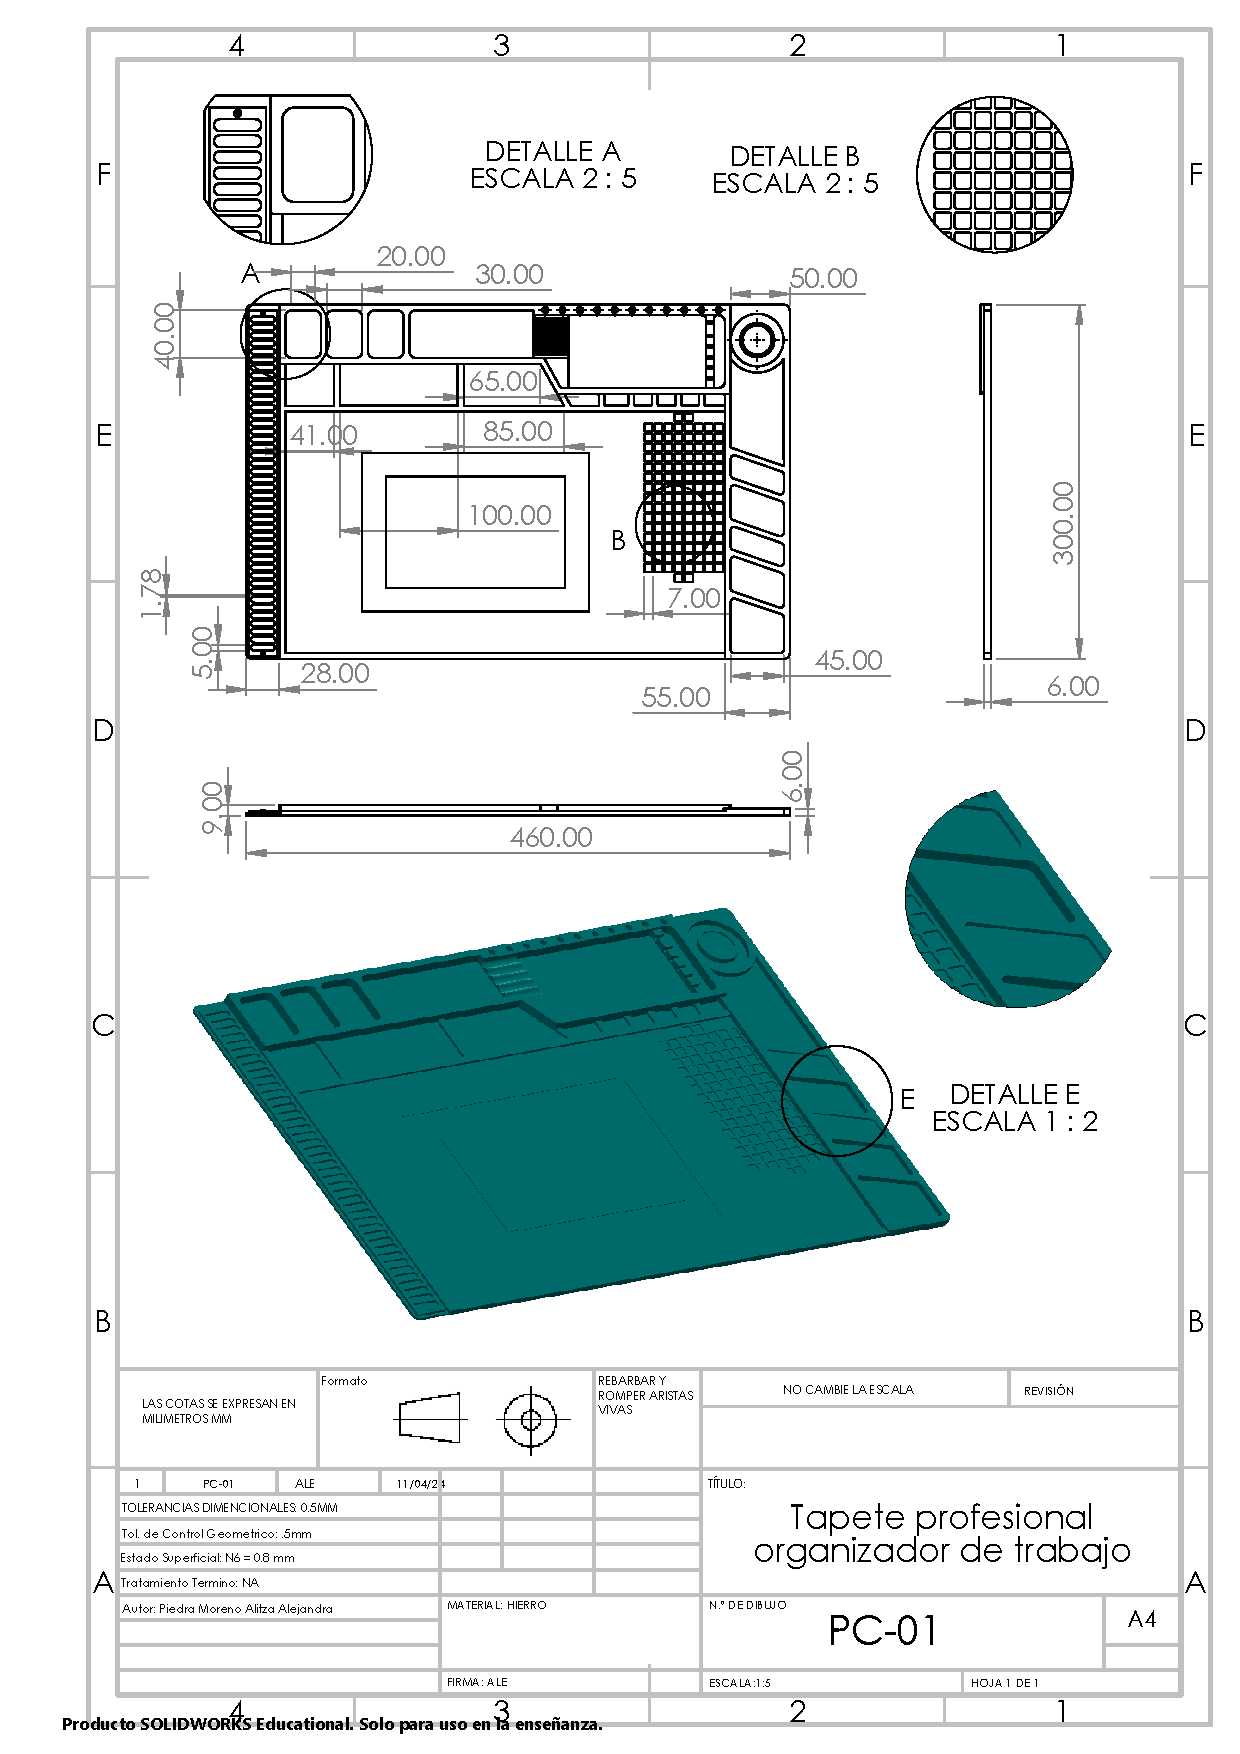
\includegraphics[trim = {7mm 1mm 1mm 1mm},clip,scale=0.4]{22/Img/almohadillaDibujo.pdf}
        \caption{Dibujo técnico de la almohadilla de trabajo}
        \label{fig:almohadillaD}
    \end{figure}
    
    Ahora que ya conocemos un poco más de la forma física de nuestro elemento, nos seguiremos a describirlo un poco más en sus propiedades, esto a razón de lo antes mencionado que es familiarizarnos primeramente con el método actual.
    
    Propiedad antiestática: Tiene áreas especiales para colocar procesadores, microchips, memorias, tarjetas de desarrollo o cualquier otro elemento de electrónica que pueda ser afectado por la estática. Incluso, te protege de las cargas estáticas almacenadas en los componentes en reposo.
    
    
    Propiedad magnética: Incorpora imanes distribuidos en lugares diferentes; perfectos para retener piezas metálicas, como tornillería, herramientas, puntas de desarmador, tarrajas y pinzas, entre otras. Además, pueden ser utilizados para magnetizar o desmagnetizar puntas de desarmadores.
    
    
    Espacios ideales para el trabajo:
    
    Mini ranuras: Perfectas para colocar las piezas de los equipos desarmados y llevar el control de su posición, gracias a que están numeradas.
    Mini cajones: Ayudan a identificar piezas pequeñas o tornillos indispensables para el reensamblaje de los equipos en reparación.
    Orificios: Útiles para que coloques tus desarmadores, aplicadores de flux o pastas en jeringa en una posición adecuada y puedas tomarlos rápidamente.
    Cajones multifunción: Estos compartimentos de diversos tamaños son apropiados para otros objetos misceláneos que utilices.
    Cajones con tapa: Adecuados para que almacenes y cuides los componentes más importantes.
    Cajones para herramientas: Tienen el espacio ideal para colocar pinzas, espátulas, punzones y más.
    Regleta: Es de 36 cm. Te servirá como referencia para trabajos en los que requieras medir.
    Espacio central: Es el área de trabajo perfecta donde puedes armar o desarmar los equipos.
    
    Material ideal para trabajar: Es flexible y tiene superficie antiderrapante. Está fabricado con silicona de textura suave al tacto que te da comodidad de uso y protege los equipos contra rayones y golpes. También puede ser usado para trabajos de soldadura, ya que soporta hasta 400 °C.
    
    
    
    \subsubsection{PC-02: Protoboard de 300 puntos}
    
    Un protoboard de 300 puntos es una placa de pruebas electrónica que se utiliza para prototipar circuitos electrónicos de manera temporal. Está diseñada con un patrón de agujeros y conexiones internas que permiten insertar y conectar componentes electrónicos de forma rápida y sin necesidad de soldadura. El “300 puntos” se refiere a la cantidad de puntos de conexión disponibles en la placa, lo que determina cuántos componentes y conexiones pueden alojarse en ella. Estos protoboards son herramientas muy útiles para diseñadores y estudiantes de electrónica, ya que les permiten experimentar y probar circuitos antes de realizar una implementación permanente.
    
    En la figura \ref{fig:proto} se muestra el diseño un tanto detallado de este elemento, como podemos ver tiene una dimensión de 55 x 82 mm, estas medidas son fundamentales a la hora de realizar nuestra distribución por lo cual necesario tenerlo en cuenta además que al tener presente que es de 300 puntos podemos destinar la posición de cada una de nuestras piezas así como optimizar nuestro ensamble.
    
    \begin{figure}[H]
        \centering
        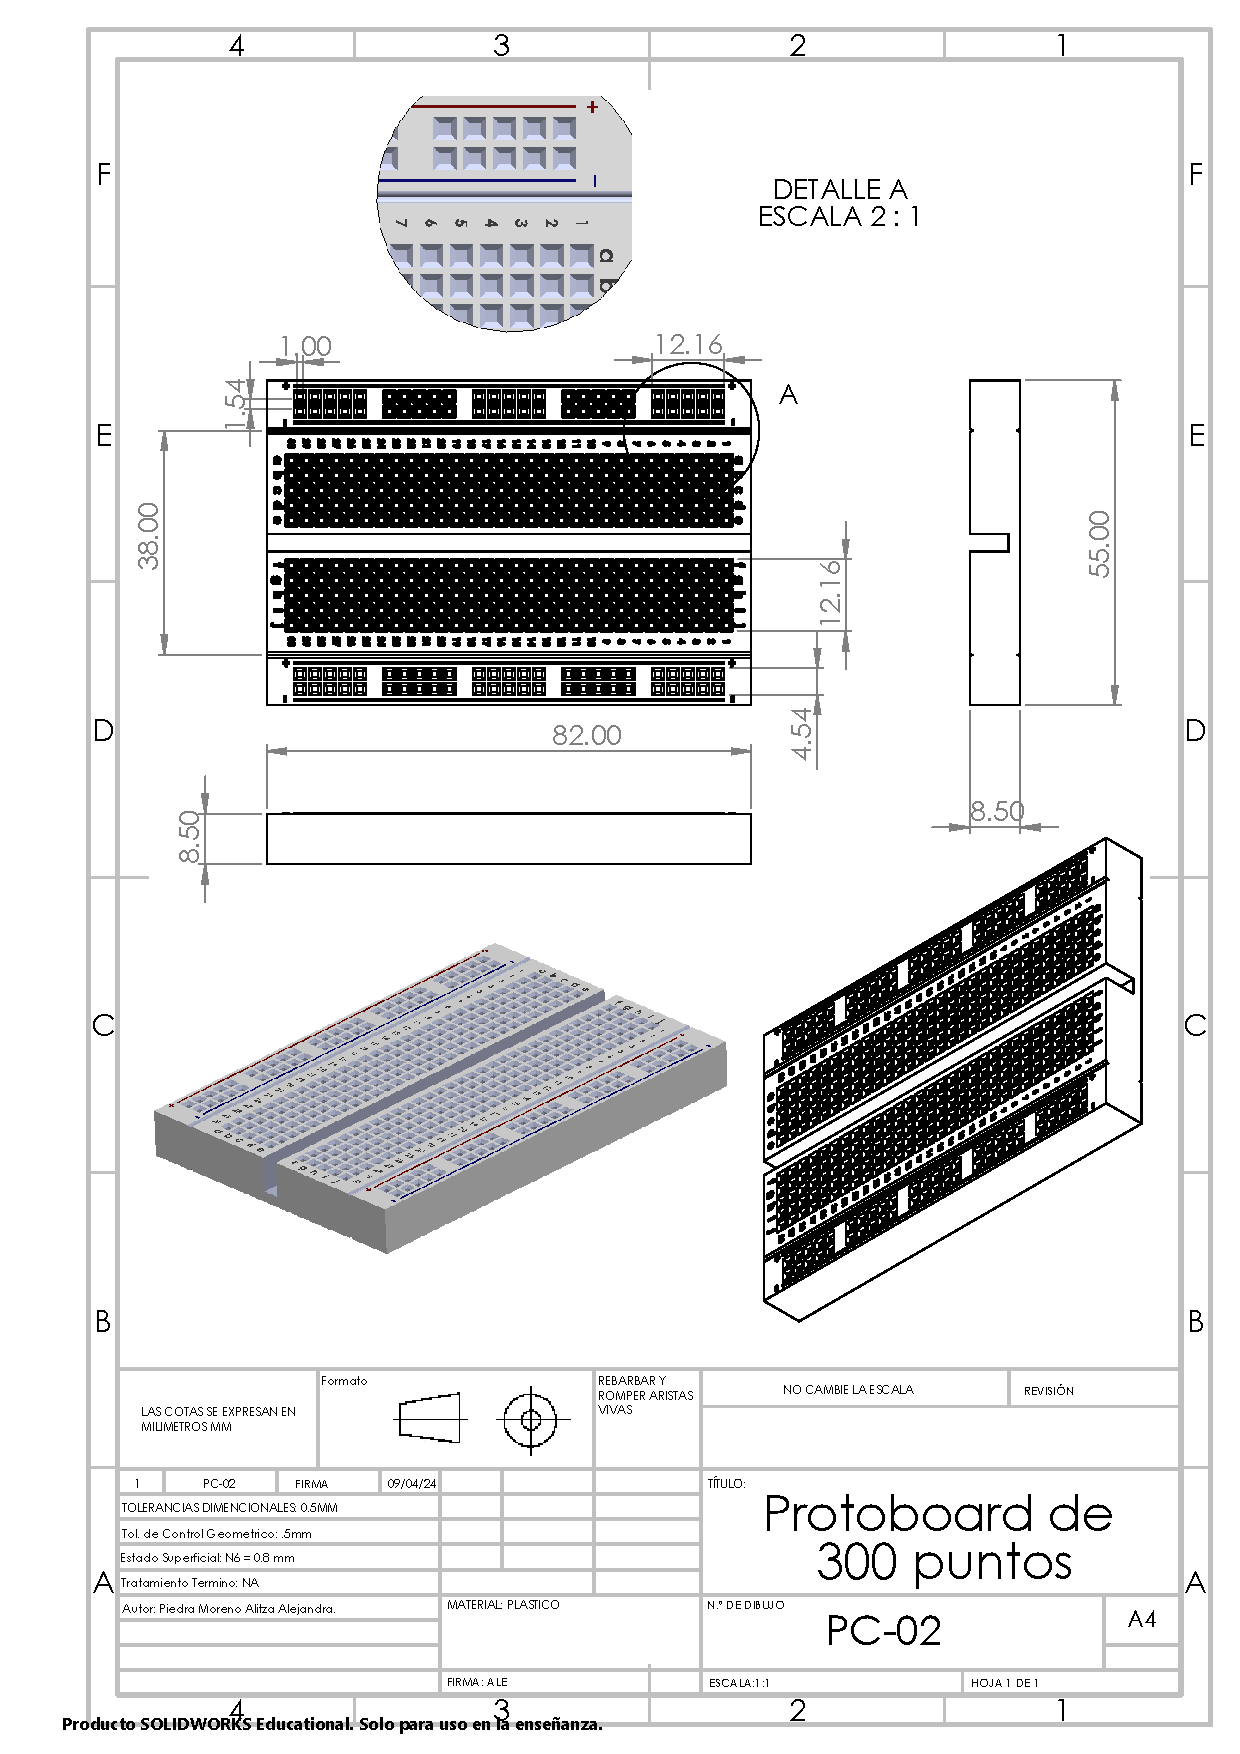
\includegraphics[trim = {7mm 1mm 1mm 1mm},clip,scale=0.4]{22/Img/protoDibujo.pdf}
        \caption{Dibujo técnico del protoboard de 300 puntos}
        \label{fig:proto}
    \end{figure}
    
    \subsubsection{PC-03: Pantalla de cristal líquido (LCD) 16X2}
    
    Una pantalla de cristal líquido (LCD) 16x2 es un tipo común de pantalla de visualización utilizada en una variedad de dispositivos electrónicos, como relojes, calculadoras, equipos de prueba, sistemas de control, y muchos otros dispositivos electrónicos. La designación “16x2” se refiere a la cantidad de caracteres que puede mostrar la pantalla en cada línea y el número de líneas, respectivamente, el 16, indica que la pantalla tiene 16 caracteres en cada línea horizontal. Esto significa que puede mostrar hasta 16 caracteres en una fila antes de pasar a la siguiente línea, mientras que el 2 indica que la pantalla tiene 2 líneas verticales de caracteres. Por lo tanto, puede mostrar dos líneas de texto o caracteres simultáneamente.
    \begin{figure}[H]
        \centering
        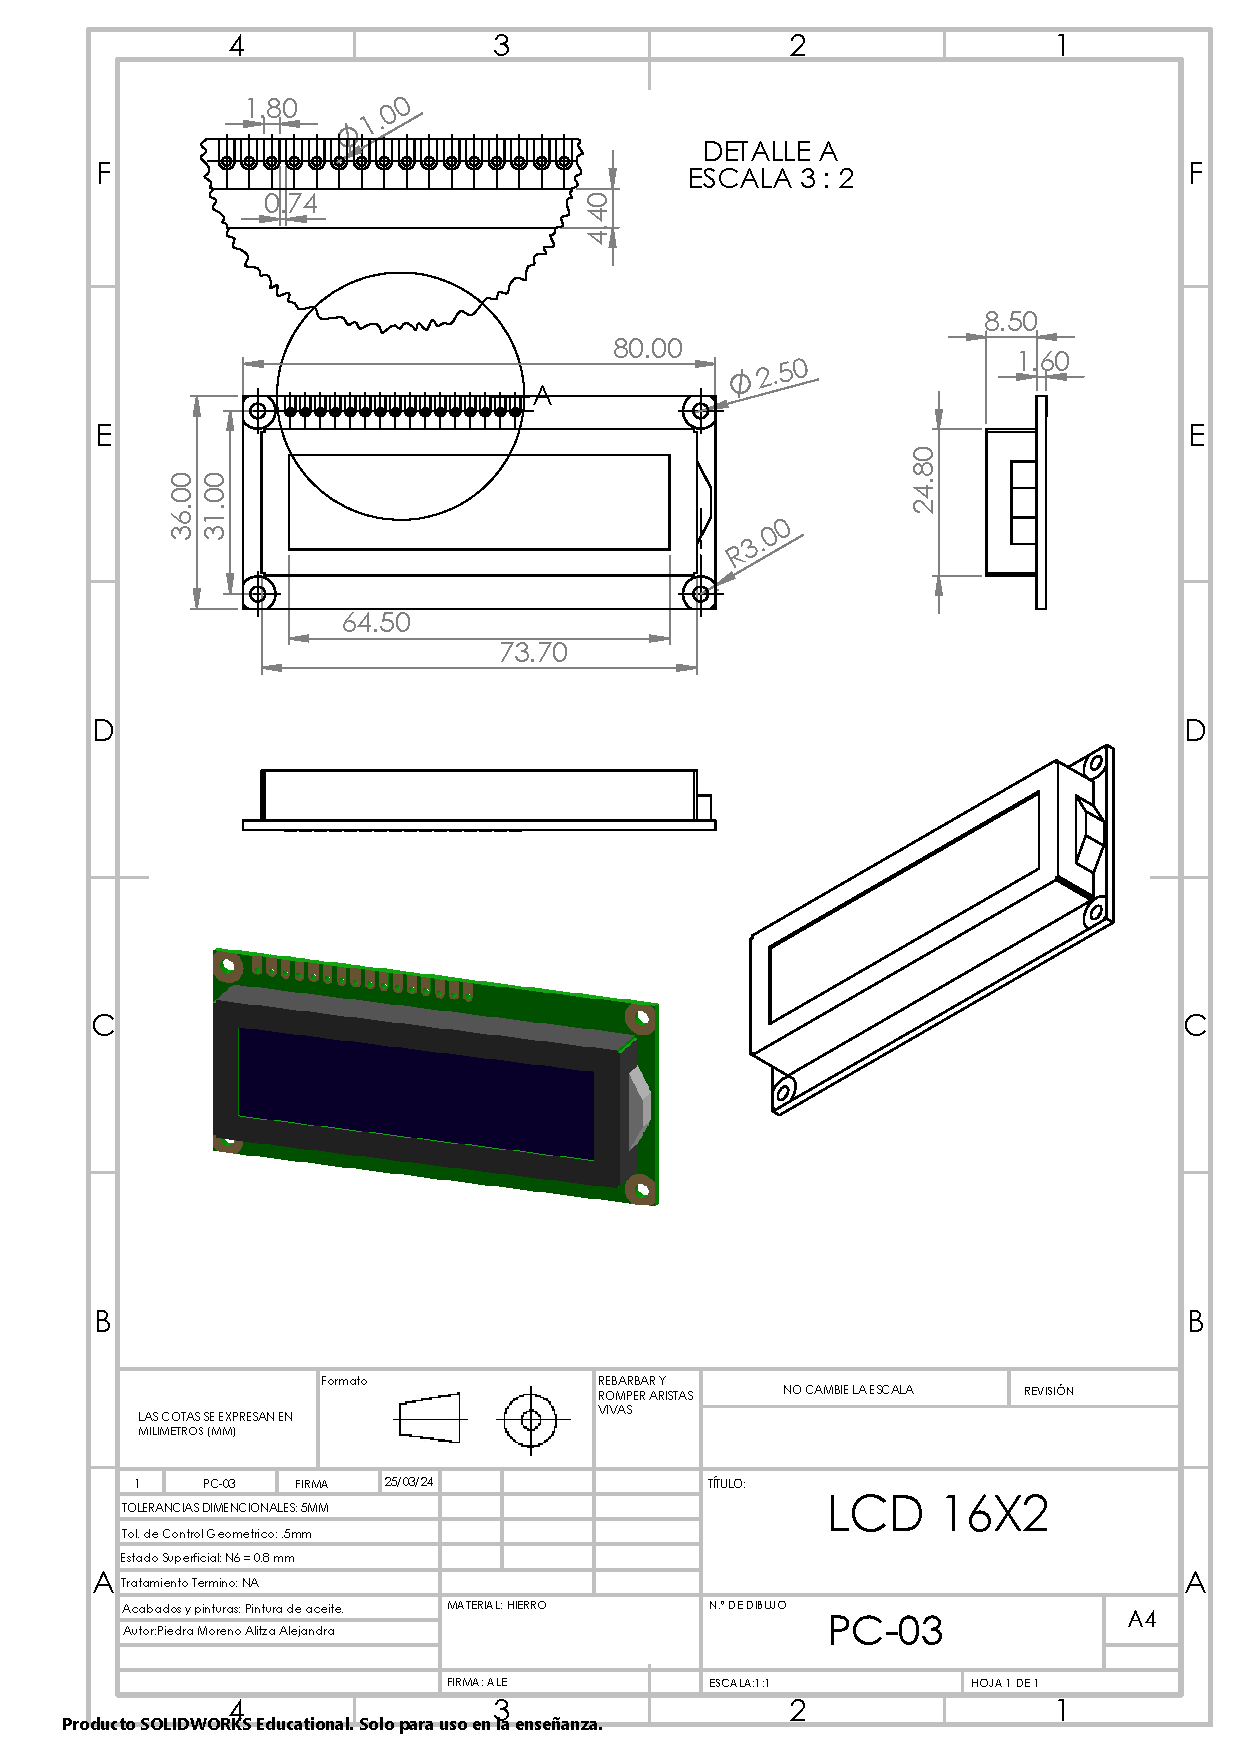
\includegraphics[trim = {7mm 1mm 1mm 1mm},clip,scale=0.4]{22/Img/lcdDibujo.PDF}
        \caption{Dibujo técnico de una LCD 16X2}
        \label{fig:lcd}
    \end{figure}
    
    Las pantallas LCD 16x2 generalmente funcionan con un controlador que facilita la comunicación con un microcontrolador o un dispositivo de procesamiento similar. Estas pantallas están compuestas por un conjunto de segmentos de cristal líquido que se activan eléctricamente para mostrar caracteres alfanuméricos, símbolos y otros tipos de información visual. Las pantallas LCD son populares debido a su bajo consumo de energía y su capacidad para mostrar información de manera clara y legible en una variedad de condiciones de iluminación.
    
    
    En la figura \ref{fig:lcd} se muestra el dibujo técnico de esta pantalla LCD, donde nos muestra dimensiones importantes que se deben tener en cuenta en nuestro análisis. Como se observa, la placa base de la lcd tiene una dimensión de 80x36 mm, además que podemos observar que contiene 16 pines o patitas que son las que nos permite mandarle señales a nuestra pantalla y a través de la interfaz esta tarea se nos facilita muchísimo más.
    
    
    
    \subsubsection{PC-04: Módulo I2C Interfaz LCD 16x2 }
    
    El módulo I2C Interfaz LCD 16x2 es un dispositivo que combina una pantalla LCD alfanumérica de 16 caracteres por 2 líneas con un controlador integrado y una interfaz de comunicación I2C. Este tipo de módulos se utilizan comúnmente en proyectos de electrónica y sistemas embebidos para proporcionar una interfaz de usuario visual.
    
    El funcionamiento del módulo I2C Interfaz LCD 16x2 es relativamente simple:
    
    Conexión física: El módulo se conecta a un microcontrolador u otro dispositivo maestro a través de dos cables: uno para la línea de datos (SDA) y otro para la línea de reloj (SCL) del bus I2C. Estas conexiones permiten que el microcontrolador envíe comandos y datos al módulo LCD.
    
    Inicialización: Antes de poder utilizar la pantalla LCD, es necesario inicializarla. Esto implica configurar el controlador del LCD para que se comunique correctamente con el microcontrolador y establecer parámetros como el contraste, el brillo y la posición del cursor.
    
    Envío de datos: Una vez inicializado, el microcontrolador puede enviar comandos y datos al módulo LCD a través del bus I2C. Estos datos pueden incluir caracteres individuales para mostrar en la pantalla, comandos de control para configurar el comportamiento del LCD (como borrar la pantalla, mover el cursor, etc.), o incluso mensajes completos que deben mostrarse en la pantalla.
    
    Actualización de la pantalla: El controlador del módulo LCD se encarga de traducir los comandos y datos recibidos del microcontrolador en acciones específicas en la pantalla. Esto puede incluir la activación y desactivación de píxeles individuales para mostrar caracteres, la actualización de la posición del cursor en la pantalla, o cualquier otra operación necesaria para reflejar los datos enviados por el microcontrolador en la pantalla LCD.
    
    En la figura \ref{fig:modulo} se muestran las medidas y detalles importantes que se deben conocer de este módulo de LCD
    \begin{figure}[H]
        \centering
        \includegraphics[trim = {7mm 1mm 1mm 1mm},clip,scale=0.4]{22/Img/móduloI2CInterfazDibujo.pdf}
        \caption{Dibujo técnico: Módulo I2C Interfaz LCD 16x2}
        \label{fig:modulo}
    \end{figure}
    
    
    \subsubsection{PC-05: ESP32-C6-WROOM-1 }
    
    El ESP32-C6-WROOM-1 es un módulo de conectividad WiFi y Bluetooth fabricado por Espressif Systems. Forma parte de la familia de microcontroladores ESP32, que son muy populares en el mundo de la electrónica y la Internet de las cosas (IoT) debido a su potencia, versatilidad y bajo costo.
    \begin{figure}[H]
        \centering
        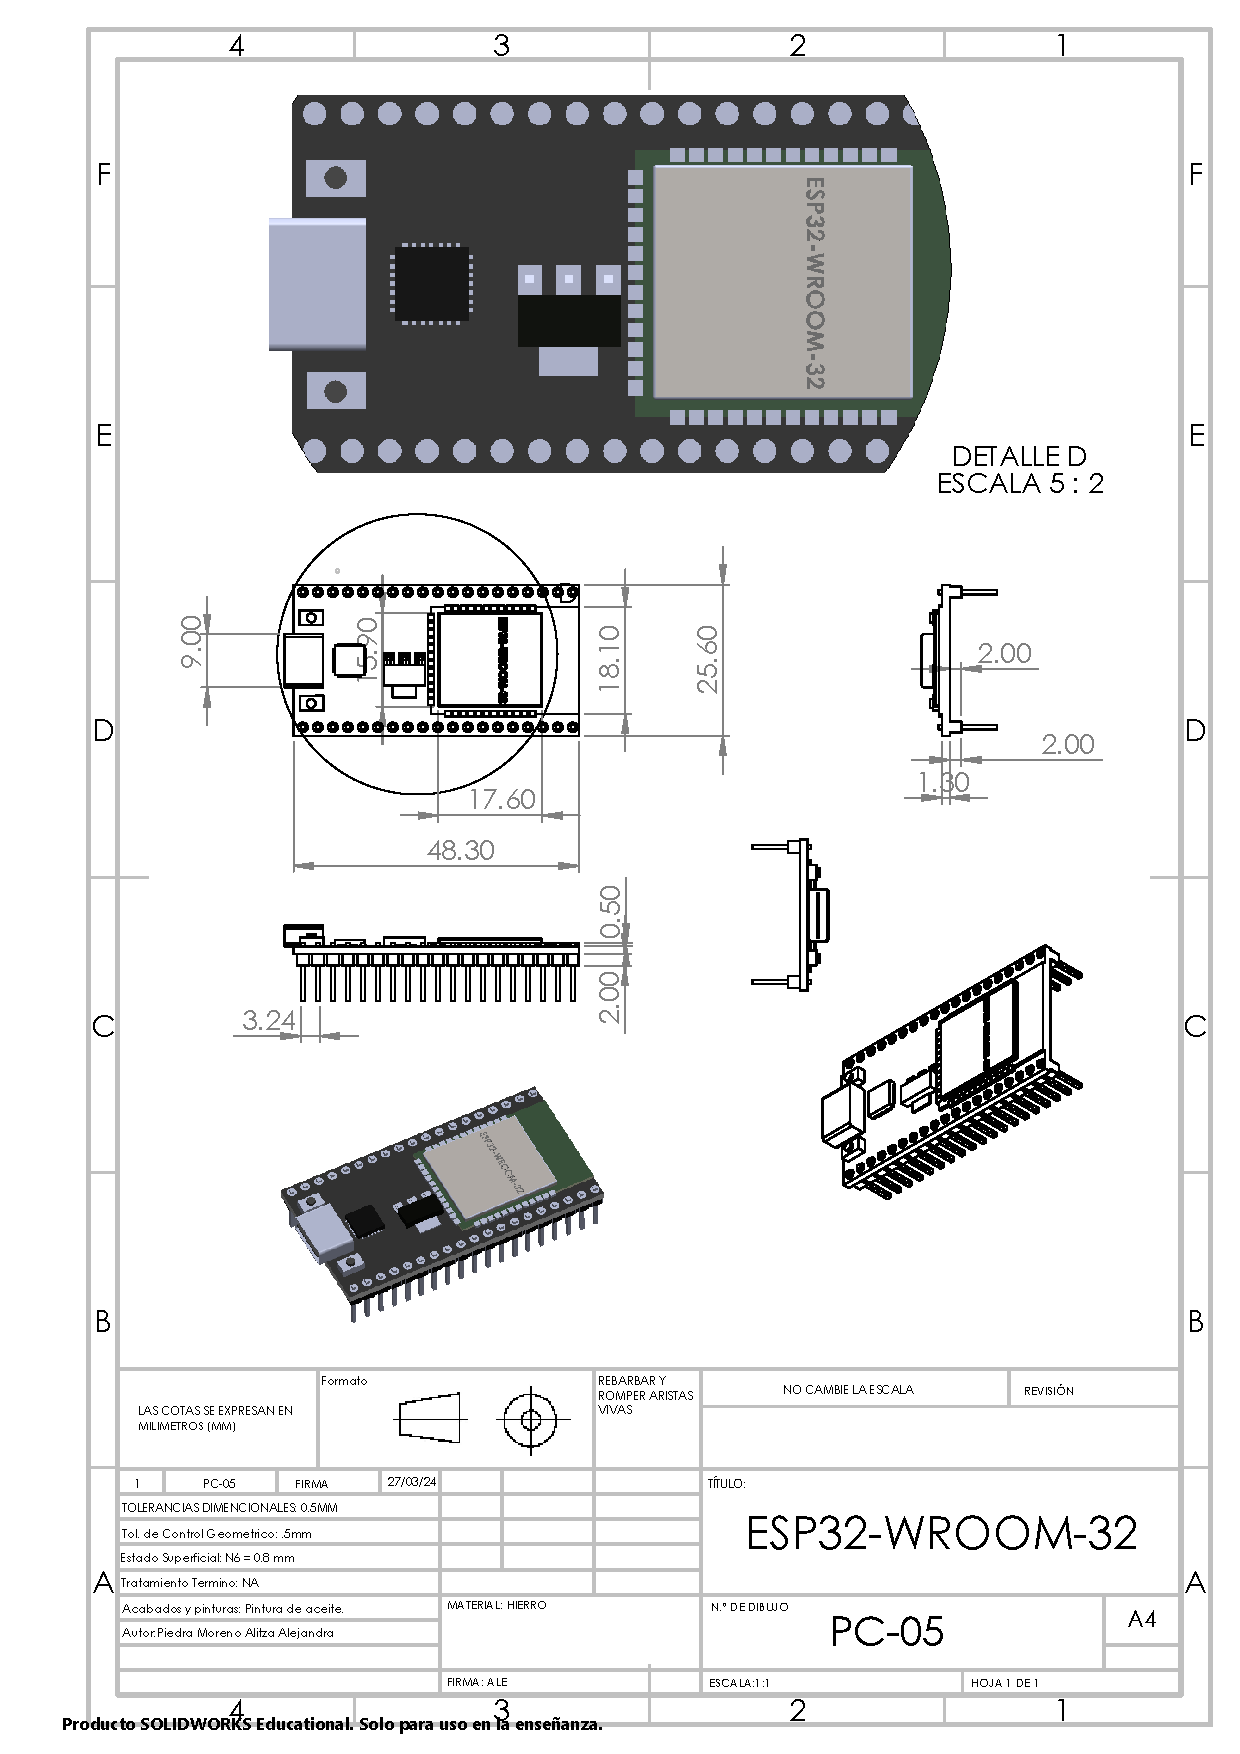
\includegraphics[trim = {7mm 1mm 1mm 1mm},clip,scale=0.4]{22/Img/esp32Dibujo.pdf}
        \caption{Dibujo técnico: ESP32-C6-WROOM-1}
        \label{fig:esp}
    \end{figure}
    
    Aquí hay algunas características clave del ESP32 WROOM 32:
    
    1. Conectividad WiFi: El módulo ofrece conectividad WiFi de doble banda (2.4 GHz y 5 GHz), lo que permite la comunicación inalámbrica con redes locales y acceso a Internet.
    
    2. Conectividad Bluetooth: Además del Wifi, el ESP32 WROOM 32 también admite Bluetooth Classic y Bluetooth de baja energía (BLE), lo que lo hace adecuado para aplicaciones que requieren interacción inalámbrica con dispositivos cercanos, como teléfonos inteligentes, sensores, entre otros.
    
    3. Procesador potente: El ESP32 WROOM 32 está equipado con un potente procesador de aplicación Tensilica Xtensa de 32 bits, que proporciona el poder de procesamiento necesario para ejecutar aplicaciones complejas y manejar múltiples tareas simultáneamente.
    
    4. Memoria integrada: El módulo cuenta con una cantidad suficiente de memoria flash y RAM integrada para almacenar el firmware del sistema, datos de la aplicación y variables temporales durante la ejecución del programa.
    
    5. Interfaces de periféricos: Ofrece una amplia gama de interfaces de periféricos, como UART, SPI, I2C, I2S, PWM, ADC, DAC, etc., que permiten la conexión con una variedad de sensores, actuadores y otros dispositivos externos.
    
    6. Seguridad: El ESP32-C6-WROOM-1 incluye características de seguridad como Secure Boot, Flash Encryption y cifrado de datos para garantizar la integridad y confidencialidad de los datos transmitidos y almacenados.
    
    En resumen, el ESP32-C6-WROOM-1 es un módulo altamente integrado y versátil que proporciona conectividad WiFi y Bluetooth junto con un potente procesador y una variedad de interfaces de periféricos, lo que lo hace ideal para una amplia gama de aplicaciones IoT y proyectos de electrónica. Para que el operario se familiarice, como en las demás piezas, en la figura \ref{fig:esp} se muestra el dibujo técnico de nuestra pieza.
    
    
    
    \subsubsection{PC-06: Potenciómetro lineal 1k preciso }
    
    Un potenciómetro es un dispositivo conformado por 2 resistencias en serie, las cuales poseen valores que pueden ser modificados por el usuario. 
    
    En la figura \ref{fig:potenciometro} encontramos el dibujo técnico del potenciómetro que se usa en la operación con sus respectivas medidas y cotas.
    
    \begin{figure}[H]
        \centering
        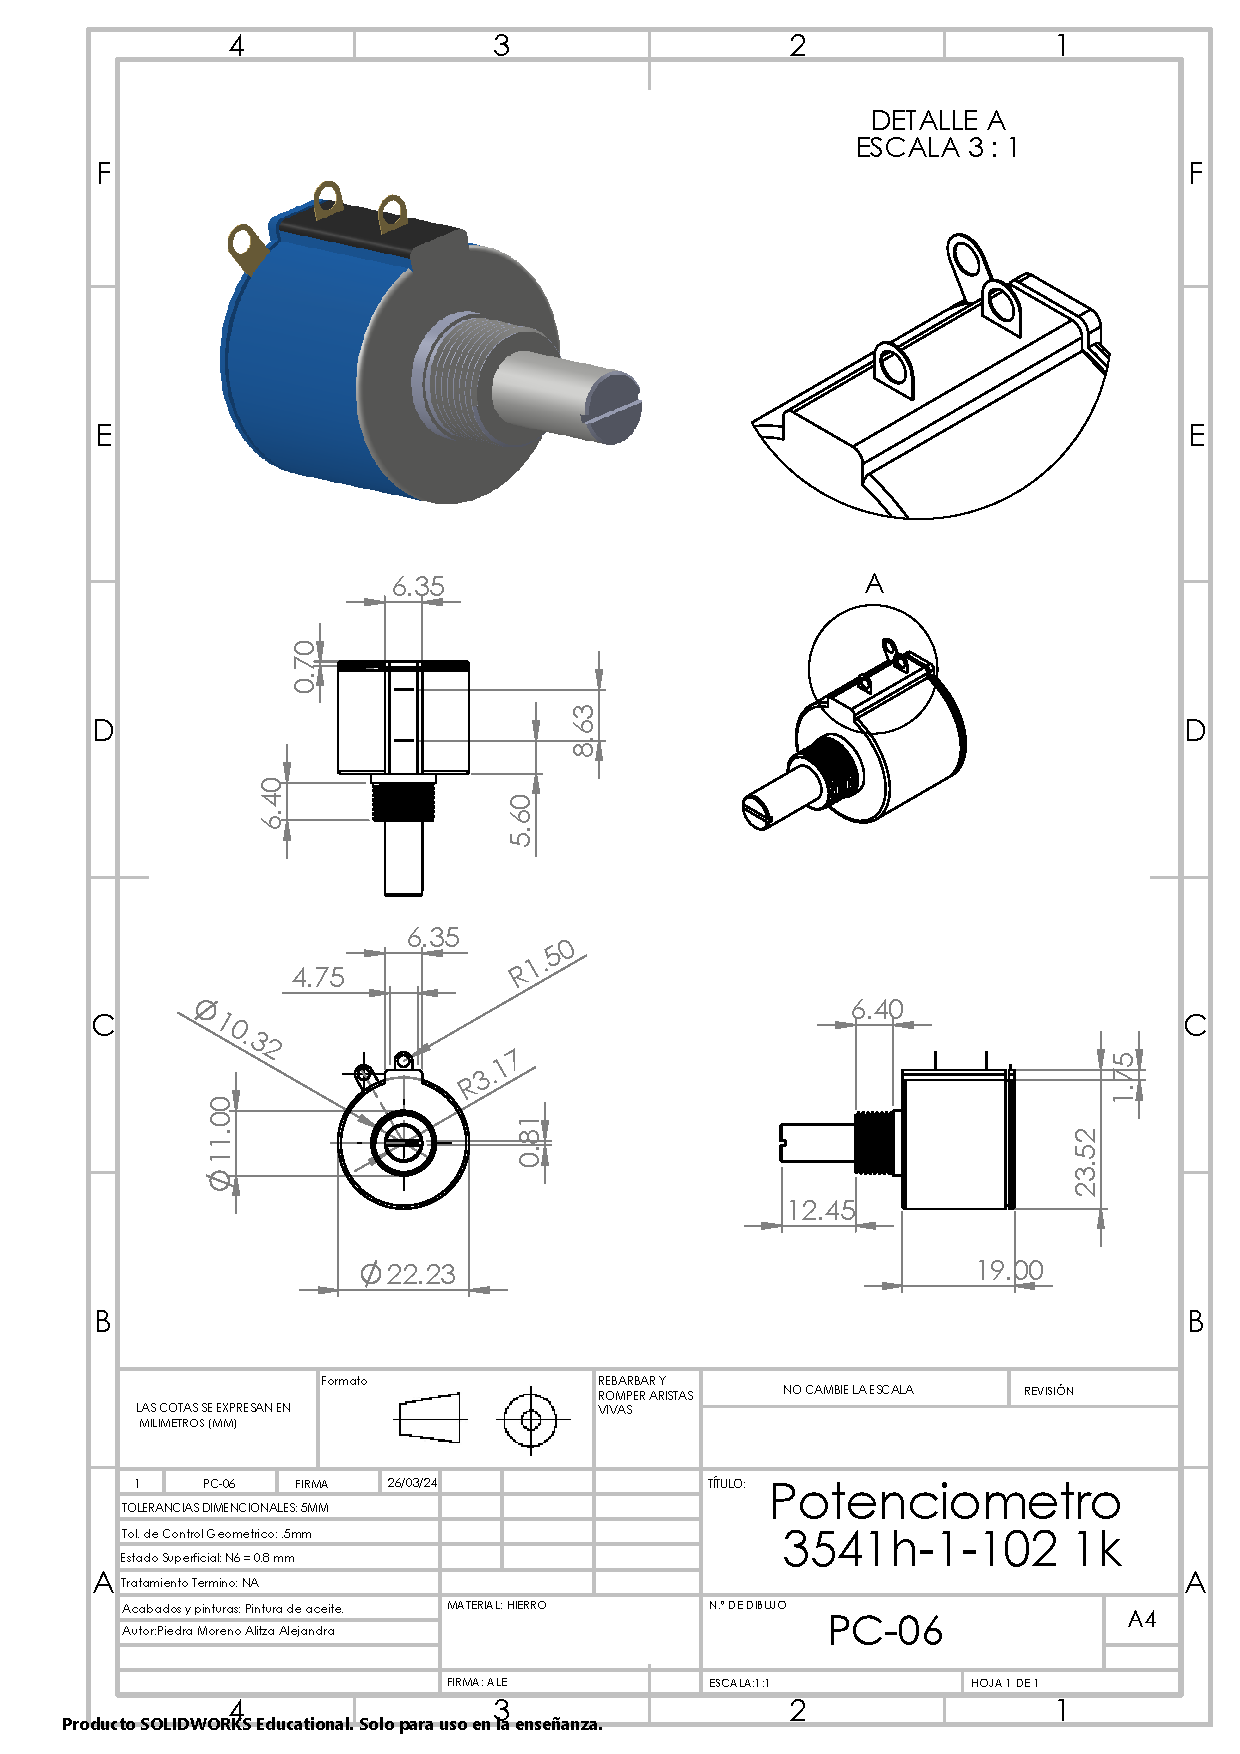
\includegraphics[trim = {7mm 1mm 1mm 1mm},clip,scale=0.4]{22/Img/potenciometroDibujo.PDF}
        \caption{Dibujo técnico: Potenciómetro lineal 1k preciso}
        \label{fig:potenciometro}
    \end{figure}
    
    
    \subsubsection{PC-07: Resistencia de 330 ohms 1/4 W }
    La resistencia es una medida de la oposición al flujo de corriente en un circuito eléctrico. La resistencia se mide en ohmios, que se simbolizan con la letra griega omega ($\Omega$). Se denominaron ohmios en honor a Georg Simon Ohm (1784-1854), un físico alemán que estudió la relación entre voltaje, corriente y resistencia. Se le atribuye la formulación de la ley de Ohm.
    
    
    
    
    
    Todos los materiales resisten en cierta medida el flujo de corriente. Se incluyen en una de dos amplias categorías:
    
    Conductores: materiales que ofrecen muy poca resistencia, donde los electrones pueden moverse fácilmente. Ejemplos: plata, cobre, oro y aluminio.
    Aislantes: materiales que presentan alta resistencia y restringen el flujo de electrones. Ejemplos: goma, papel, vidrio, madera y plástico.
    Normalmente, se toman las mediciones de resistencia para indicar las características de un componente o un circuito.
    \begin{figure}[H]
        \centering
        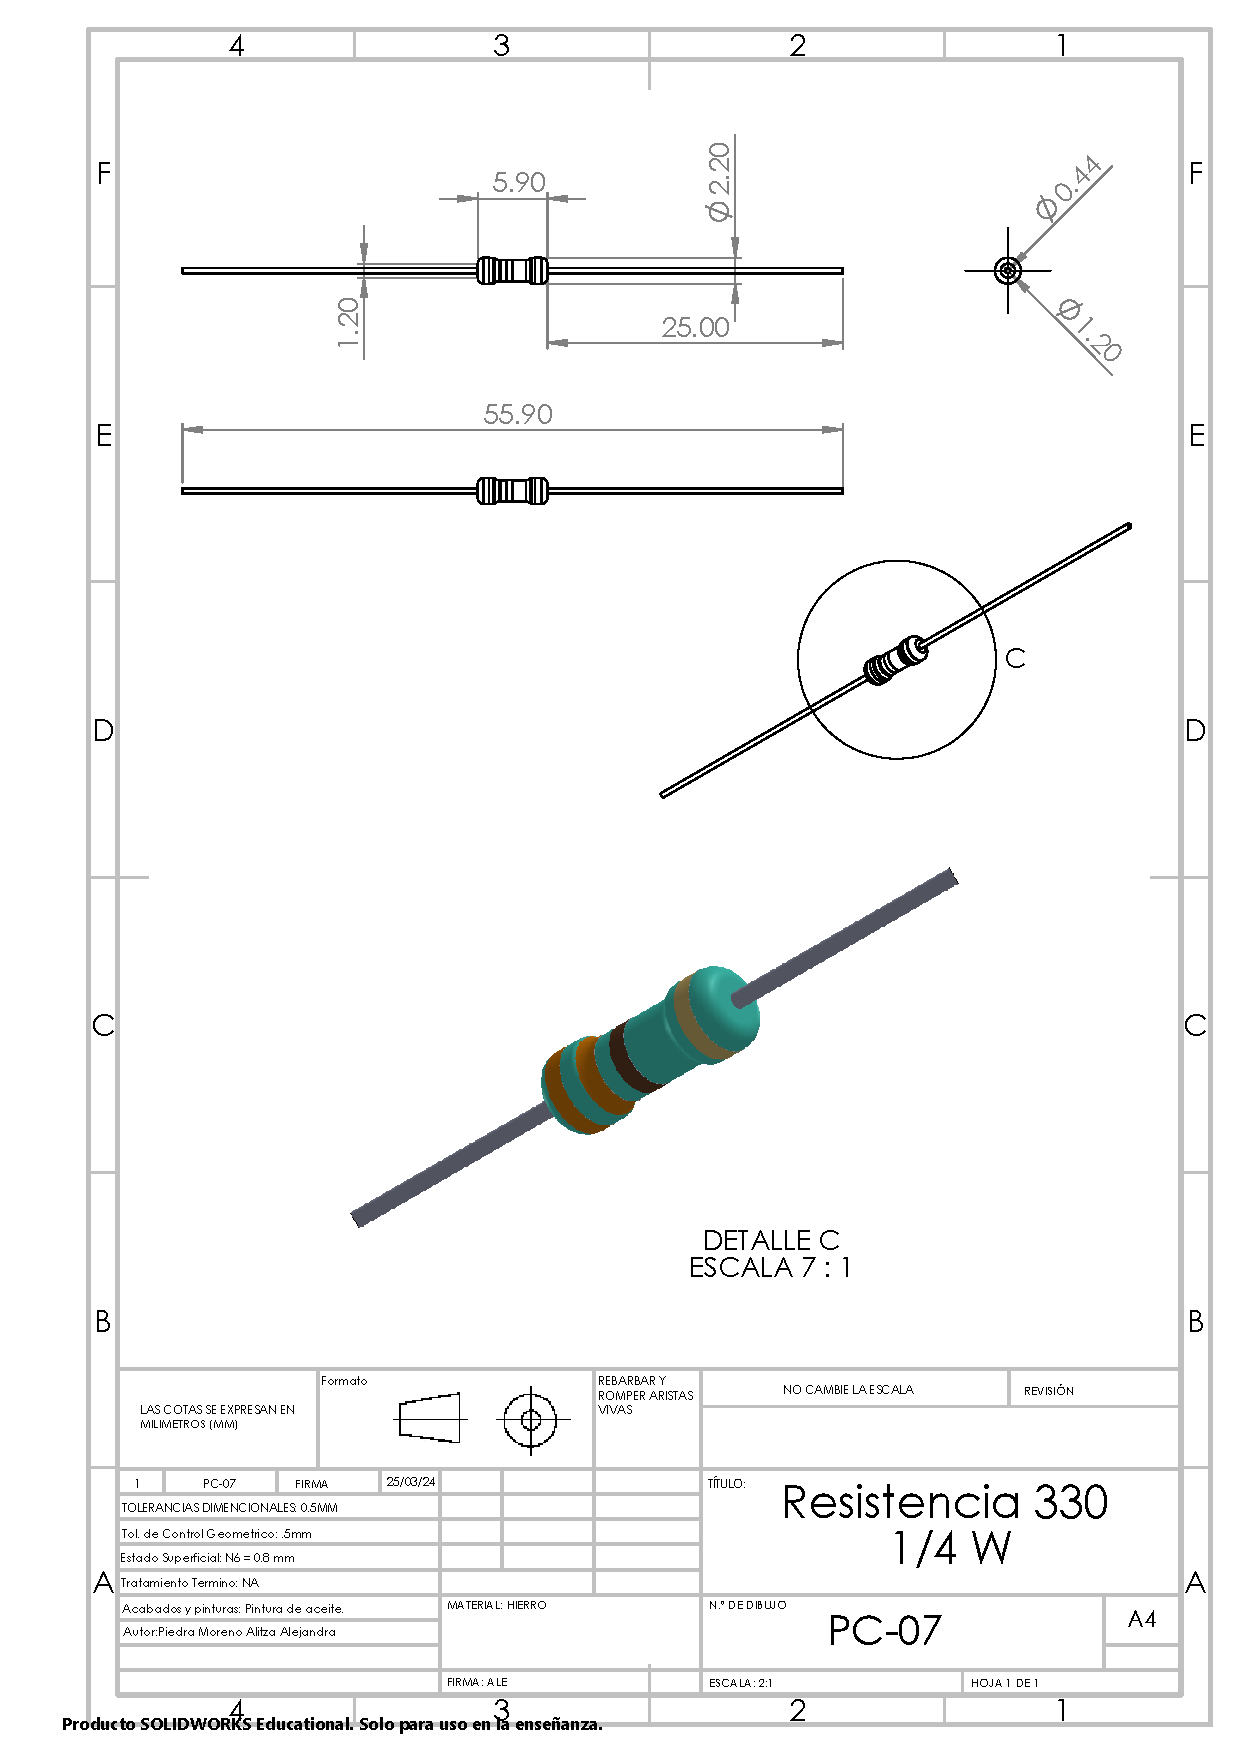
\includegraphics[trim = {7mm 1mm 1mm 1mm},clip,scale=0.4]{22/Img/resistenciaDibujo.PDF}
        \caption{Dibujo técnico: Resistencia de 330 ohms 1/4 W}
        \label{fig:resistencia}
    \end{figure}
    Cuanto mayor sea la resistencia, menor será el flujo de corriente. Si es anormalmente alta, una causa posible (entre muchas) podrían ser los conductores dañados por el fuego o la corrosión. Todos los conductores emiten cierto grado de calor, por lo que el sobrecalentamiento es un problema que a menudo se asocia con la resistencia.
    
    Cuanto menor sea la resistencia, mayor será el flujo de corriente. Causas posibles: aisladores dañados por la humedad o un sobrecalentamiento.
    Muchos componentes, tales como los elementos de calefacción y las resistencias, tienen un valor de resistencia fijo. Estos valores se imprimen a menudo en las placas de identificación de los componentes o en los manuales de referencia.
    
    Cuando se indica una tolerancia, el valor de resistencia debe encontrarse dentro de la gama de la resistencia especificada. Cualquier cambio significativo en un valor de resistencia fijo generalmente indica un problema. \cite{Fluke}
    
    
     En la figura \ref{fig:resistencia} podemos observar el dibujo técnico de nuestras residencias de 330 ohms, incluyendo sus vistas y cotas.
     \begin{figure}[H]
        \centering
        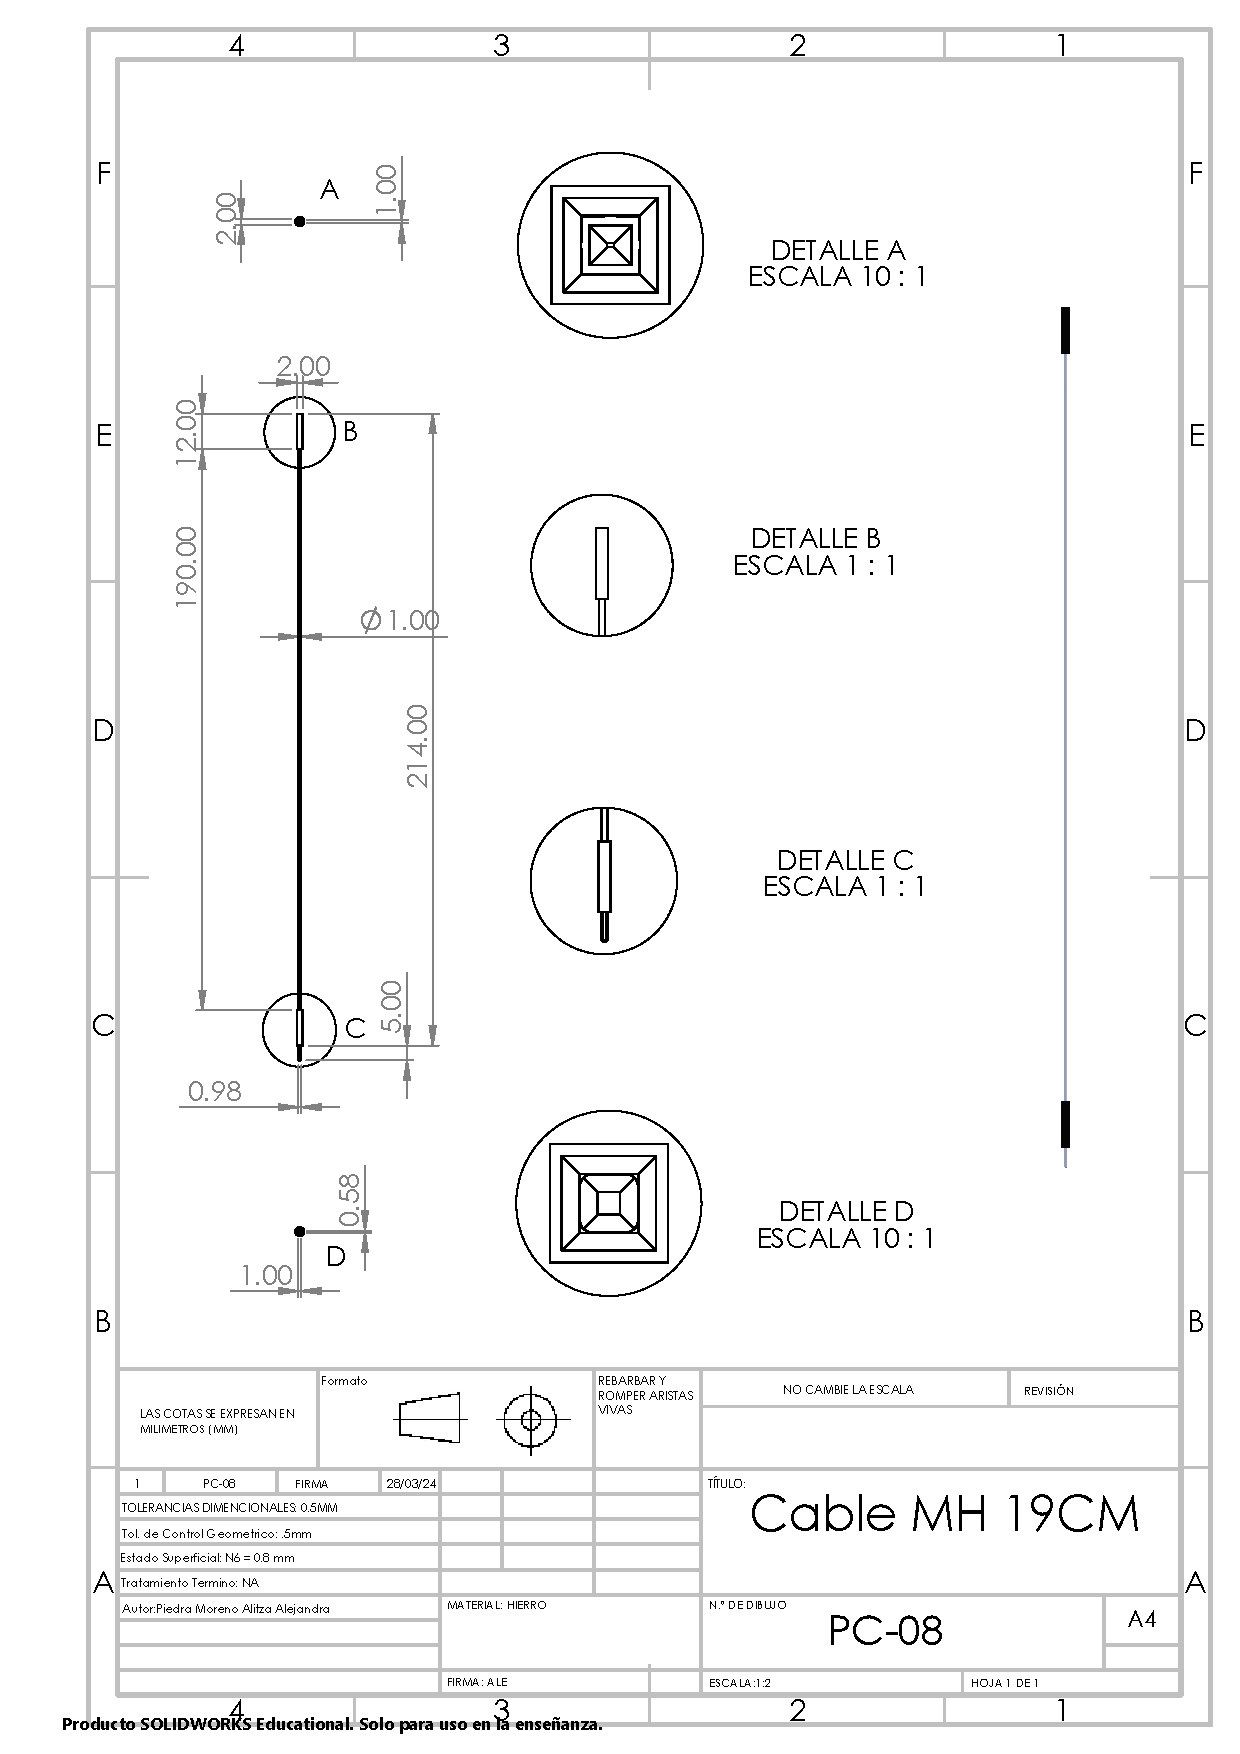
\includegraphics[trim = {7mm 1mm 1mm 1mm},clip,scale=0.4]{22/Img/cableMHDibujo.PDF}
        \caption{Dibujo técnico: Cable MH}
        \label{fig:Cable MH}
    \end{figure}
    
    \subsubsection{PC-08: Cables DuPont }
    
    Conector DuPont es un término vernáculo que se refiere a varios tipos diferentes de conectores de paso de 0,1 pulgadas. Cuentan con carcasas de plástico negro que retienen contactos con dedos integrados en el cuerpo de la carcasa. Todos son muy similares en apariencia, pero varían significativamente en calidad y precio.
    
    A menudo se les atribuyen otros nombres, como “Conector TYU” o “Conector JWT” (deje un comentario si conoce otro). Estos son acrónimos de algunos de los muchos fabricantes chinos, a veces moldeados físicamente en el producto. \cite{Mateo}
    
    Se utilizan principalmente como cables puente en protoboards y para interconectar tarjetas de desarrollo con sensores, módulos, actuadores, motores, etc. Suelen verse mucho en proyectos con Arduino o Raspberry Pi y son un material que se ha vuelto indispensable para estudiantes que trabajan con circuitos electrónicos. 
    
    Véase la figura \ref{fig:Cable MH} para observar las medidas de un cable DuPont macho-hembra de 10 cm y en la figura \ref{fig:Cable MM} para el cable mach-macho igualmente de 10 cm.
    
    
    
    \begin{figure}[H]
        \centering
        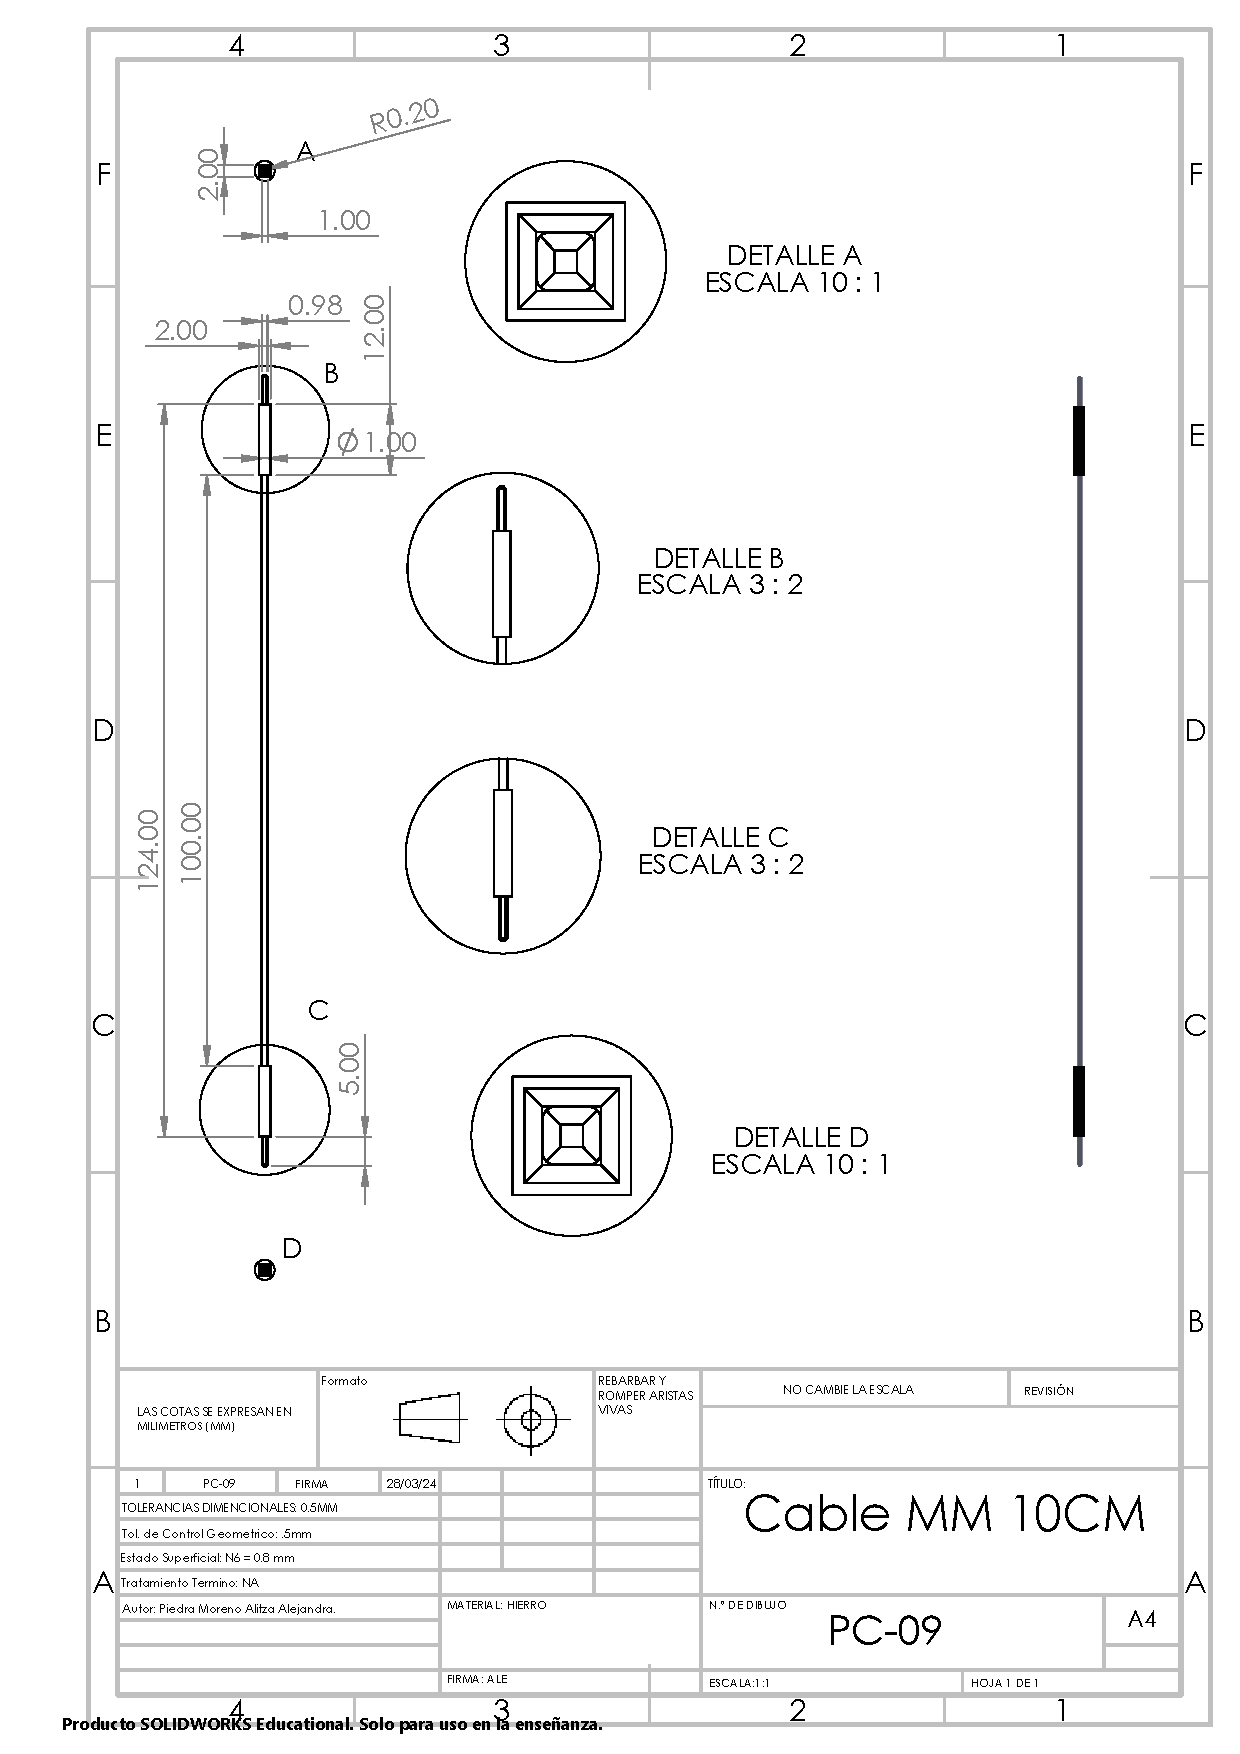
\includegraphics[trim = {7mm 1mm 1mm 1mm},clip,scale=0.4]{22/Img/cableMMDibujo.PDF}
        \caption{Dibujo técnico: Cable MM}
        \label{fig:Cable MM}
    \end{figure}
    
    \subsubsection{PC-10: Regulador Multicontacto Con 8 Salidas 3 USB Y 1 Tipo C }
    
    Las extensiones eléctricas y las barras multicontacto son útiles cuando un contacto no queda cerca del aparato que se desea conectar, o bien, no es suficiente para conectar más de dos aparatos al mismo tiempo.
    La descripción de la regleta que nosotros utilizamos es la siguiente:
    
    Regleta de alimentación con 8 salidas de CA y 4 barras de alimentación USB con protector contra sobretensiones con 8 tomas de CA y 4 puertos de carga USB (1 toma USB C) Cable de extensión de 1,2 m de alta resistencia (1625 W/13 A), protector contra sobretensiones (1700 julios) con protección contra sobrecargas que protege contra picos y fluctuaciones.
    
    Carga rápida e inteligente USB-C: 4 puertos USB 3,4 A en total, cada puerto USB A cuenta con una salida máxima de 2,4 A. El puerto de carga USB C cuenta con 3A MAX. Construido con tecnología inteligente, detecta los dispositivos de carga y ofrece una velocidad de carga óptima de forma automática, compatible con la mayoría de los dispositivos USB.
    
    NOTA: El puerto UCB-C no es compatible con ningún otro dispositivo que necesite
    salidas de protección contra sobretensiones de 8 AC con un voltaje de carga de 14 22 V: el circuito protector contra sobretensiones complementario de 3 niveles, compuesto por TVS (supresor de voltaje transitorio), con una capacidad mínima de absorción de energía de 2700 julios, podría proteger sus dispositivos mucho más de forma rápida y confiable que los circuitos de protección contra sobretensiones MOV de 1 nivel de otras marcas.
    
    Seguridad y certificado: certificación de seguridad ETL, con cable de extensión y otros componentes principales certificados por UL. El interruptor de protección contra sobrecorriente limita la corriente de trabajo de la regleta a una configuración determinada, por lo que no se calentará durante el uso. La carcasa de PC con protección ambiental y resistencia al fuego con retardante de llama a 1382 F hace que sea más duradera y tenga una vida útil más larga.
    
    Lo que obtiene: regleta, devolución en 30 días, nuestro servicio de atención al cliente confiable y sin preocupaciones de 24 meses le responderá en 24 horas.
    
    
    Para tener una noción del tamaño, véase la figura \ref{fig:multicontacto}, en donde se muestra el dibujo técnico de la pieza, y coloca las medidas correspondientes de estas, así como sus vistas.
    \begin{figure}[H]
        \centering
        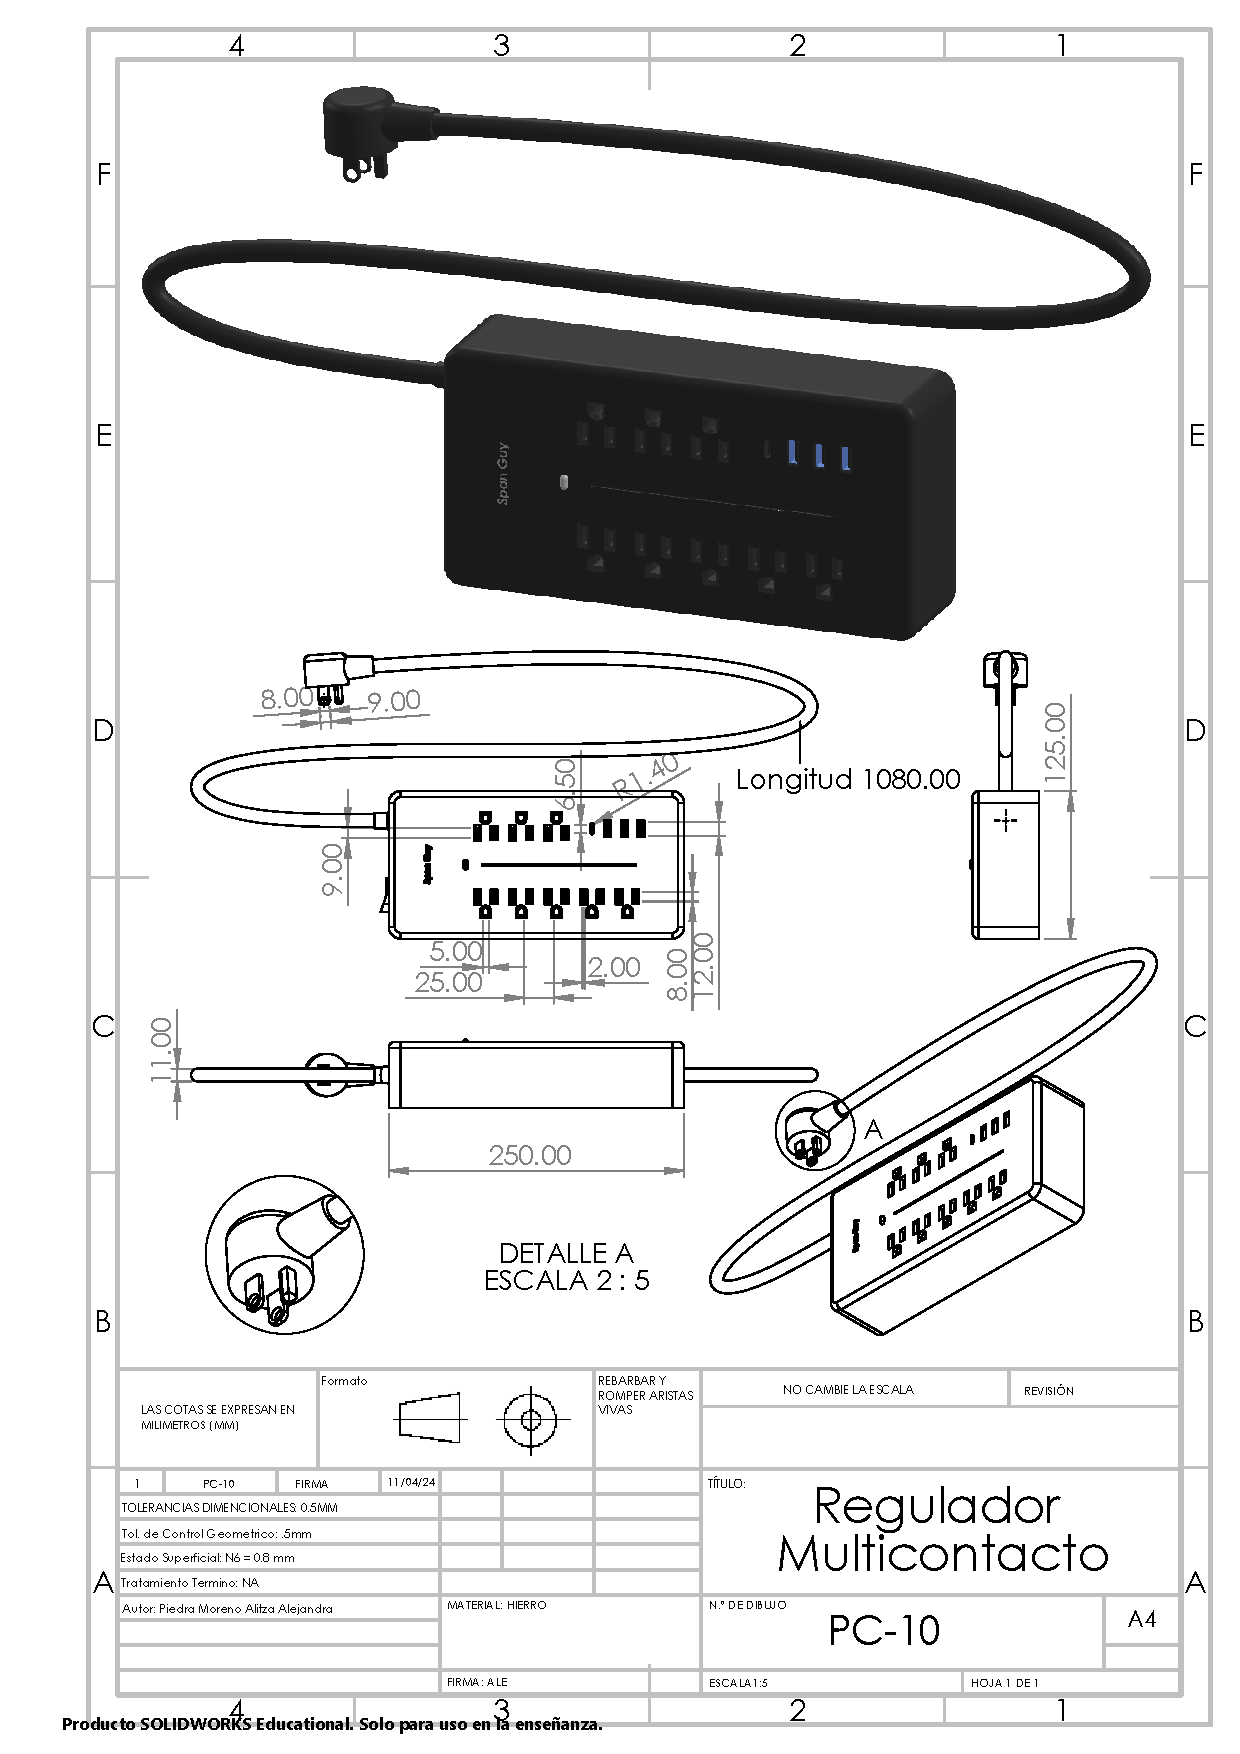
\includegraphics[trim = {7mm 1mm 1mm 1mm},clip,scale=0.4]{22/Img/multicontactoDibujo.pdf}
        \caption{Dibujo técnico: Cable MM}
        \label{fig:multicontacto}
    \end{figure}
    
    \subsubsection{PC-11: Cable Tipo C }
    Se trata de un conector de formato pequeño doble cara de 24 pines. Es conocido por facilitar la transferencia de datos y archivos de manera rápida entre diferentes dispositivos.
    
    La ventaja de este tipo de cable, es que su velocidad de transferencias es de hasta 10 GB/s. Asimismo, es capaz de proporcionar energía a través de la carga rápida, que es una tecnología adaptada a los móviles y dispositivos para alcanzar un mayor nivel de batería en menos tiempo.
    
    Para conocer más este cable véase la figura \ref{fig:cableC}, en donde podemos encontrar las medidas y vista de nuestra pieza a utilizar. 
    
    \begin{figure}[H]
        \centering
        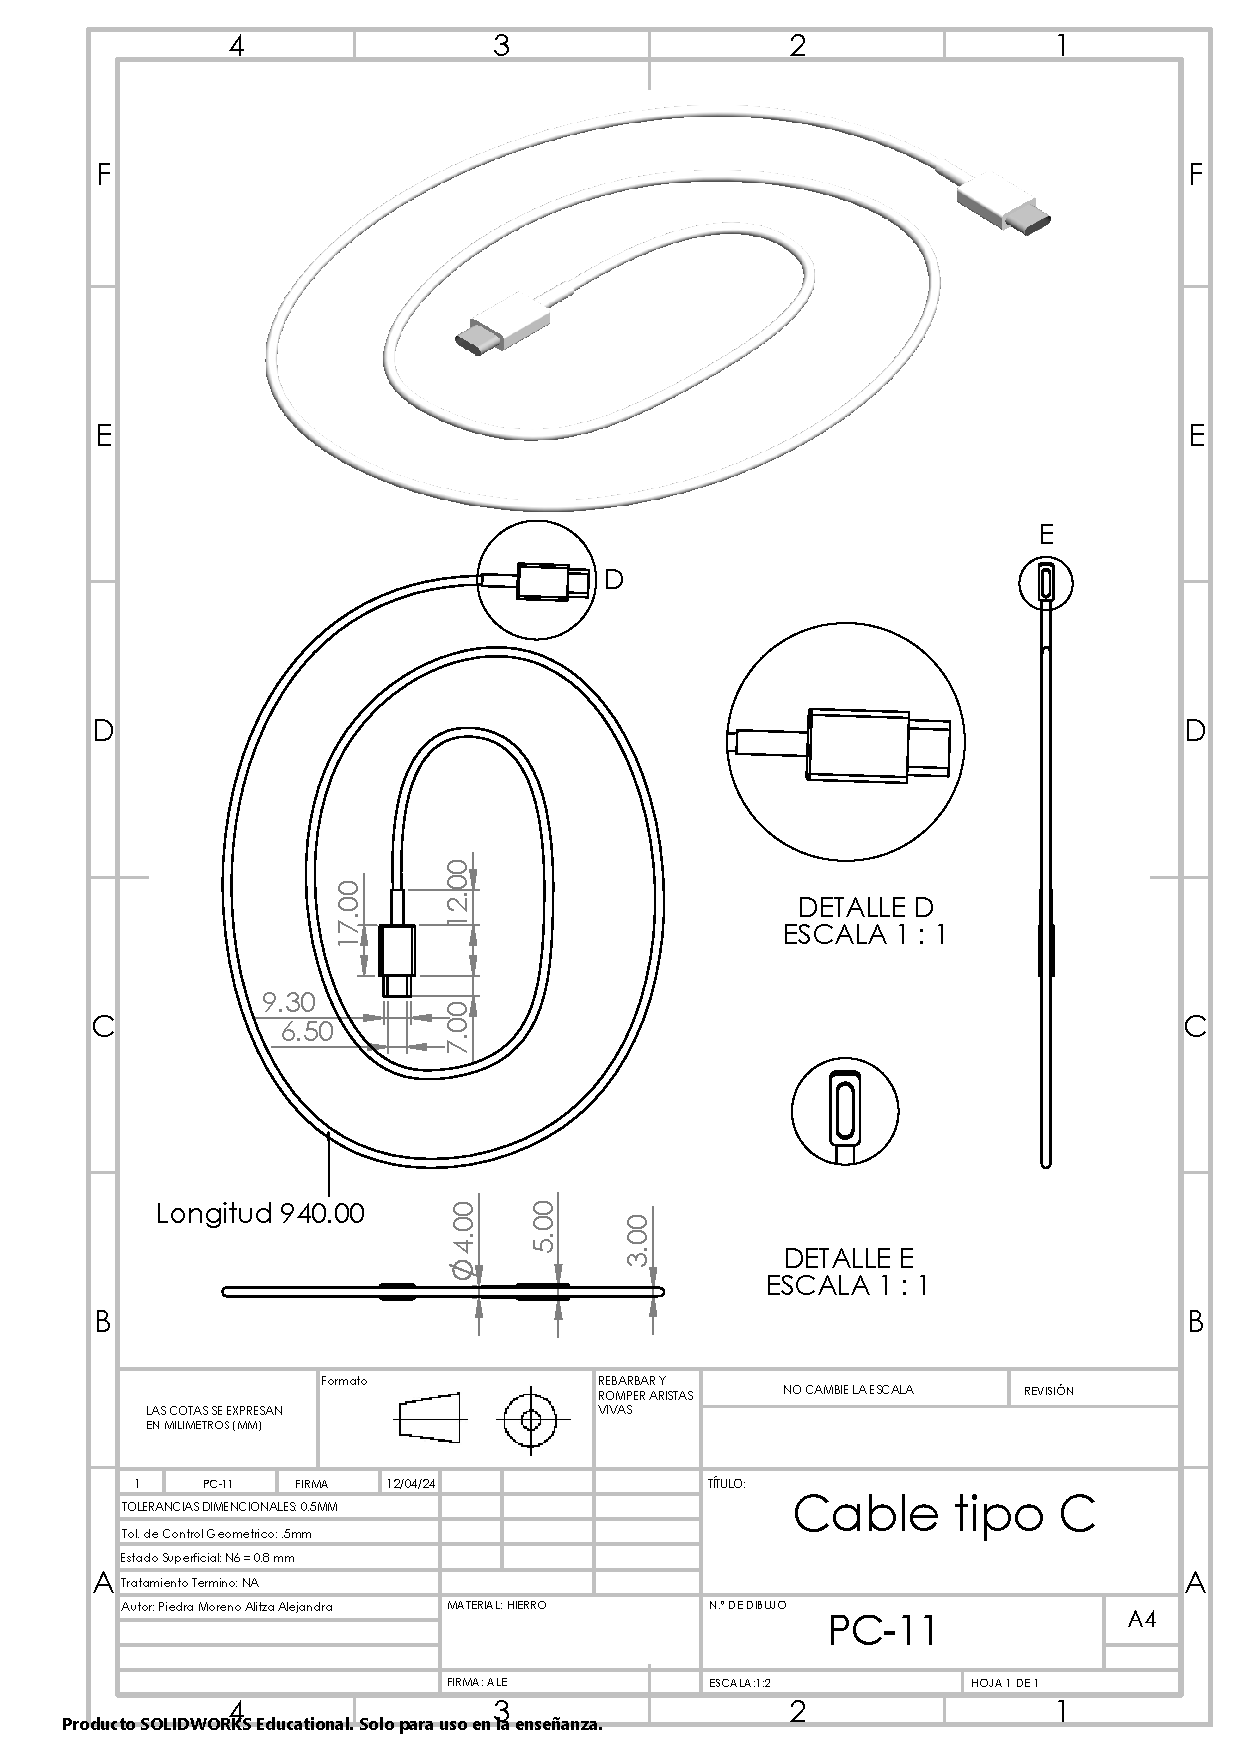
\includegraphics[trim = {7mm 1mm 1mm 1mm},clip,scale=0.4]{22/Img/cableCDibujo.PDF}
        \caption{Dibujo técnico: Cable MM}
        \label{fig:cableC}
    \end{figure}
    
    %https://www.acerstore.cl/news/usb-tipo-c-que-es-y-para-que-sirve/%
    
    
    \section{Resultados y discusión}
    
    En el desarrollo del proyecto se planteó el problema de la fata de datos como lo son la media y la varianza de nuestra población, los cuales en nuestro análisis forman una parte fundamental para llegar a nuestros resultados. Para ello se implementó varios métodos, uno de ellos es con el uso de las probabilidades, en donde para obtener la media poblacional se usó la ecuación \ref{equ:media} y para  la desviación estándar utilizamos la ecuación \ref{equ:des}
        \begin{equation}
            \label{equ:media}
           \mu = \dfrac{b+a}{2}
        \end{equation}
    
      \begin{equation}
            \label{equ:des}
            \sigma = \sqrt{\dfrac{(b-a+1)^2-1}{12}}
        \end{equation}
    
    
    
    En las siguientes figuras se muestran la evidencias del primer muestreo, el cual se realizó el día 3 de mayo del 2024, el salón C08, en el Instituto Tecnológico campus Querétaro.
    
       
    \begin{figure}[H]
        \centering
        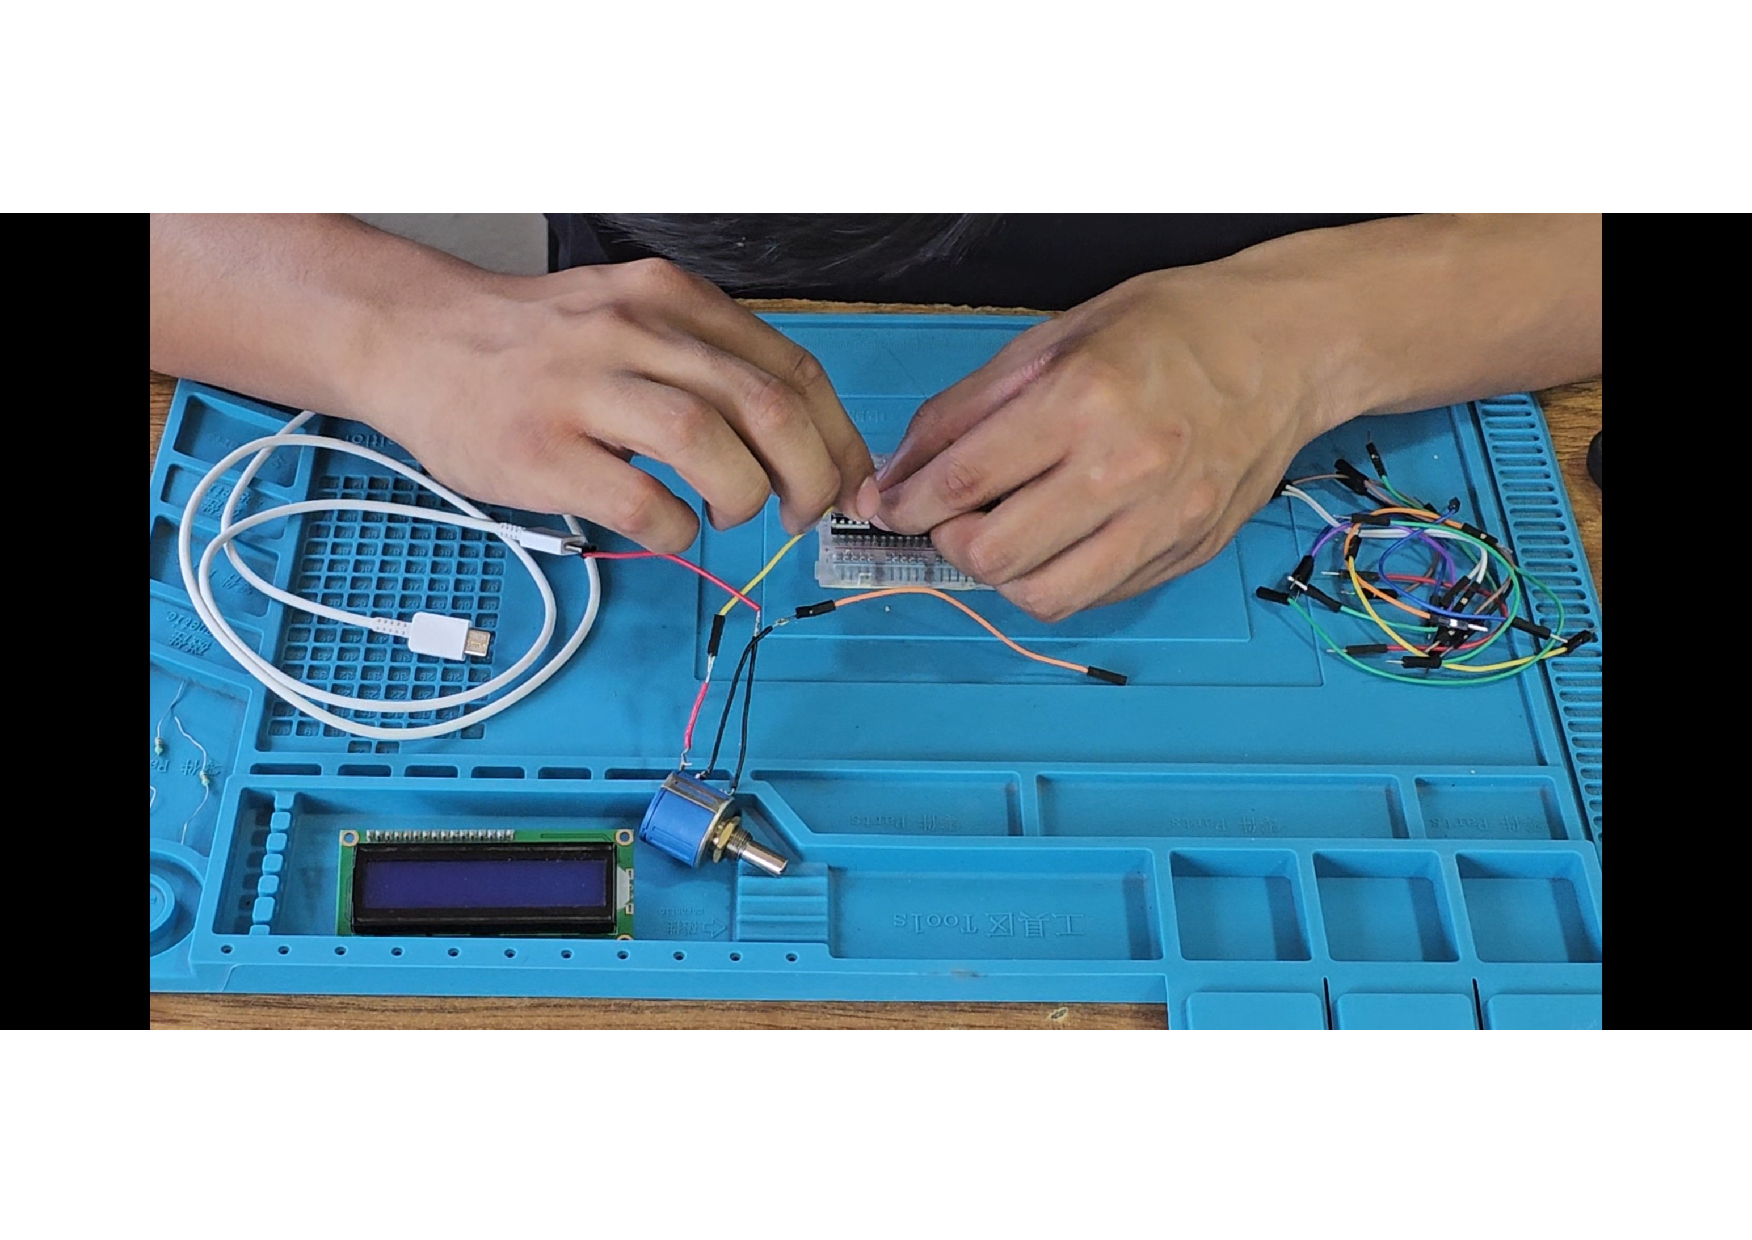
\includegraphics[trim = {7mm 1mm 1mm 1mm},clip,scale=0.25]{22/Img/e2.pdf}
        \caption{Inicio de la operación}
        \label{fig:evi1}
    \end{figure}
    
    \begin{figure}[H]
        \centering
        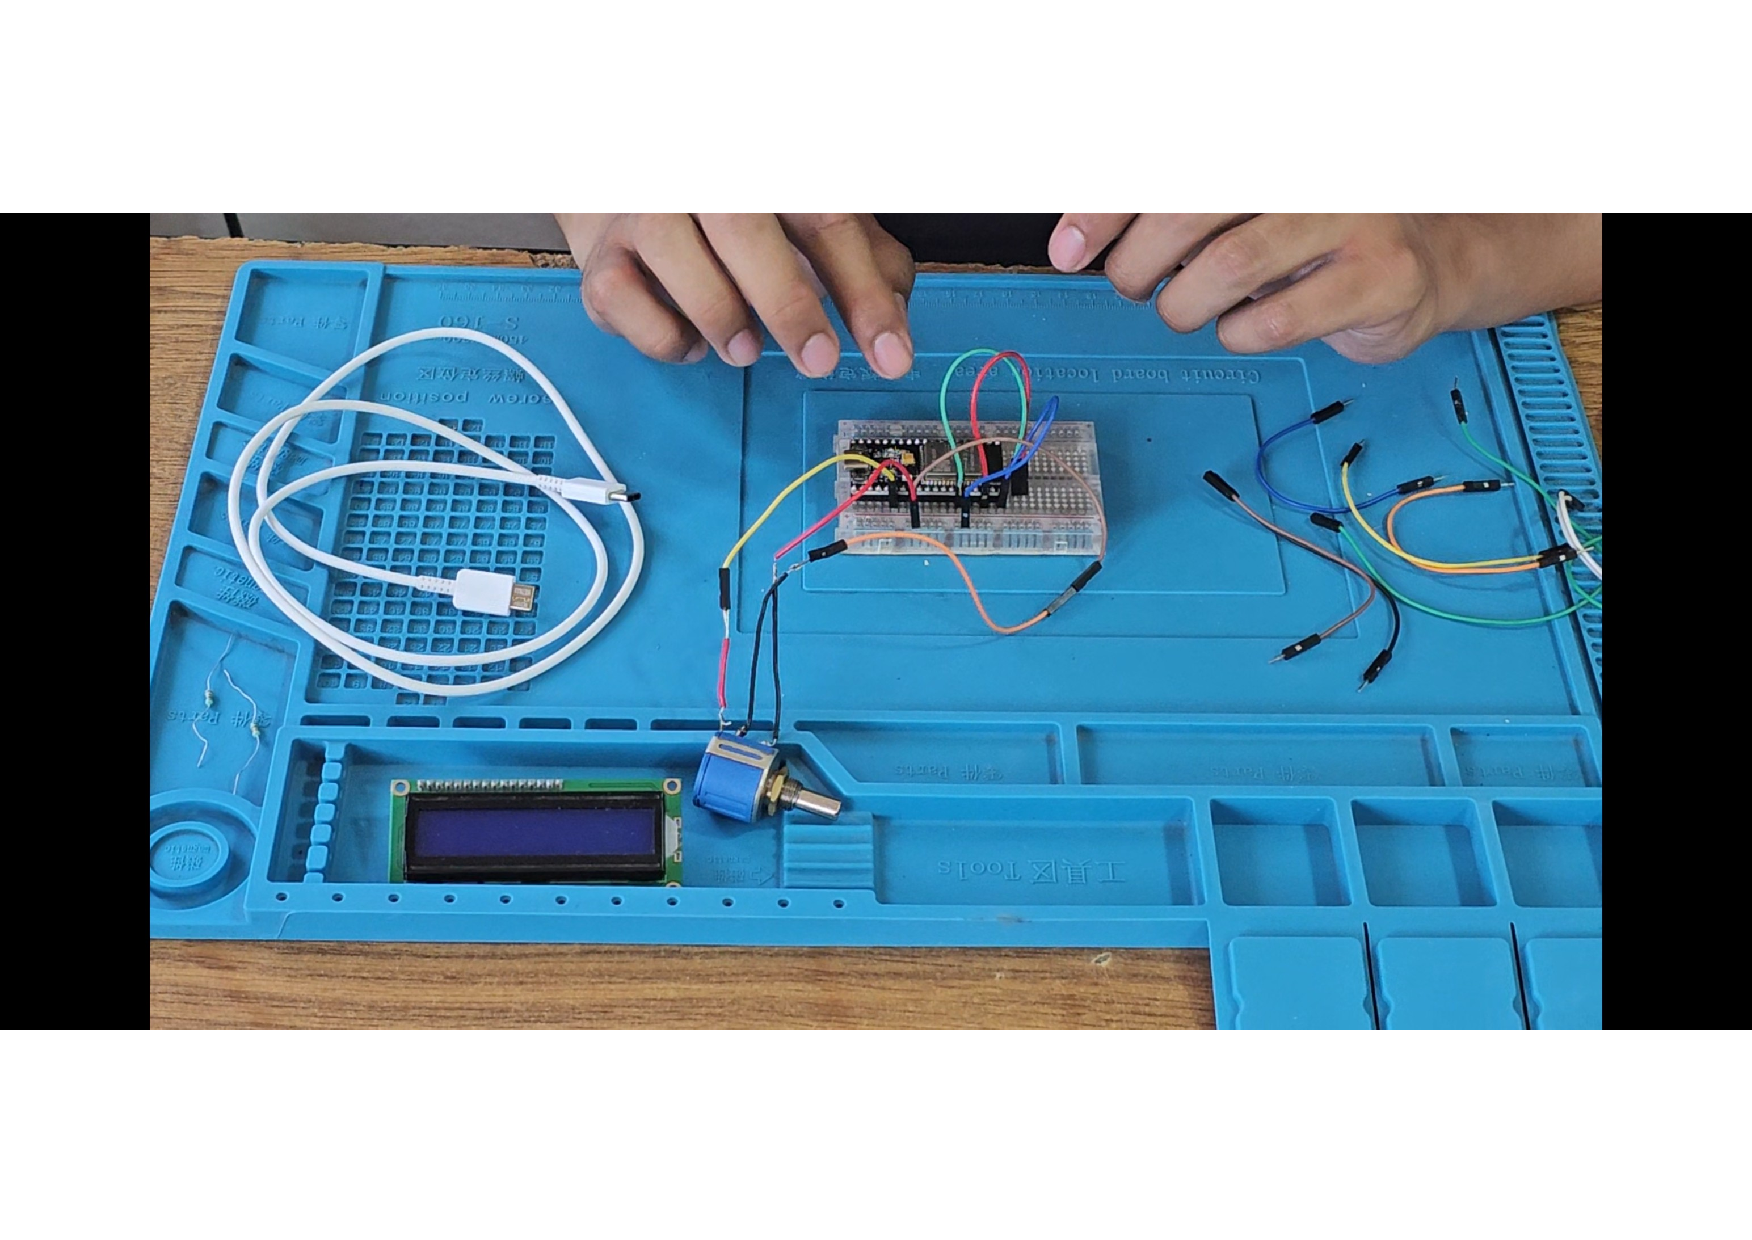
\includegraphics[trim = {7mm 1mm 1mm 1mm},clip,scale=0.25]{22/Img/e5.pdf}
        \caption{Operación a mitad de la secuencia}
        \label{fig:evi2}
    \end{figure}
    
    \begin{figure}[H]
        \centering
        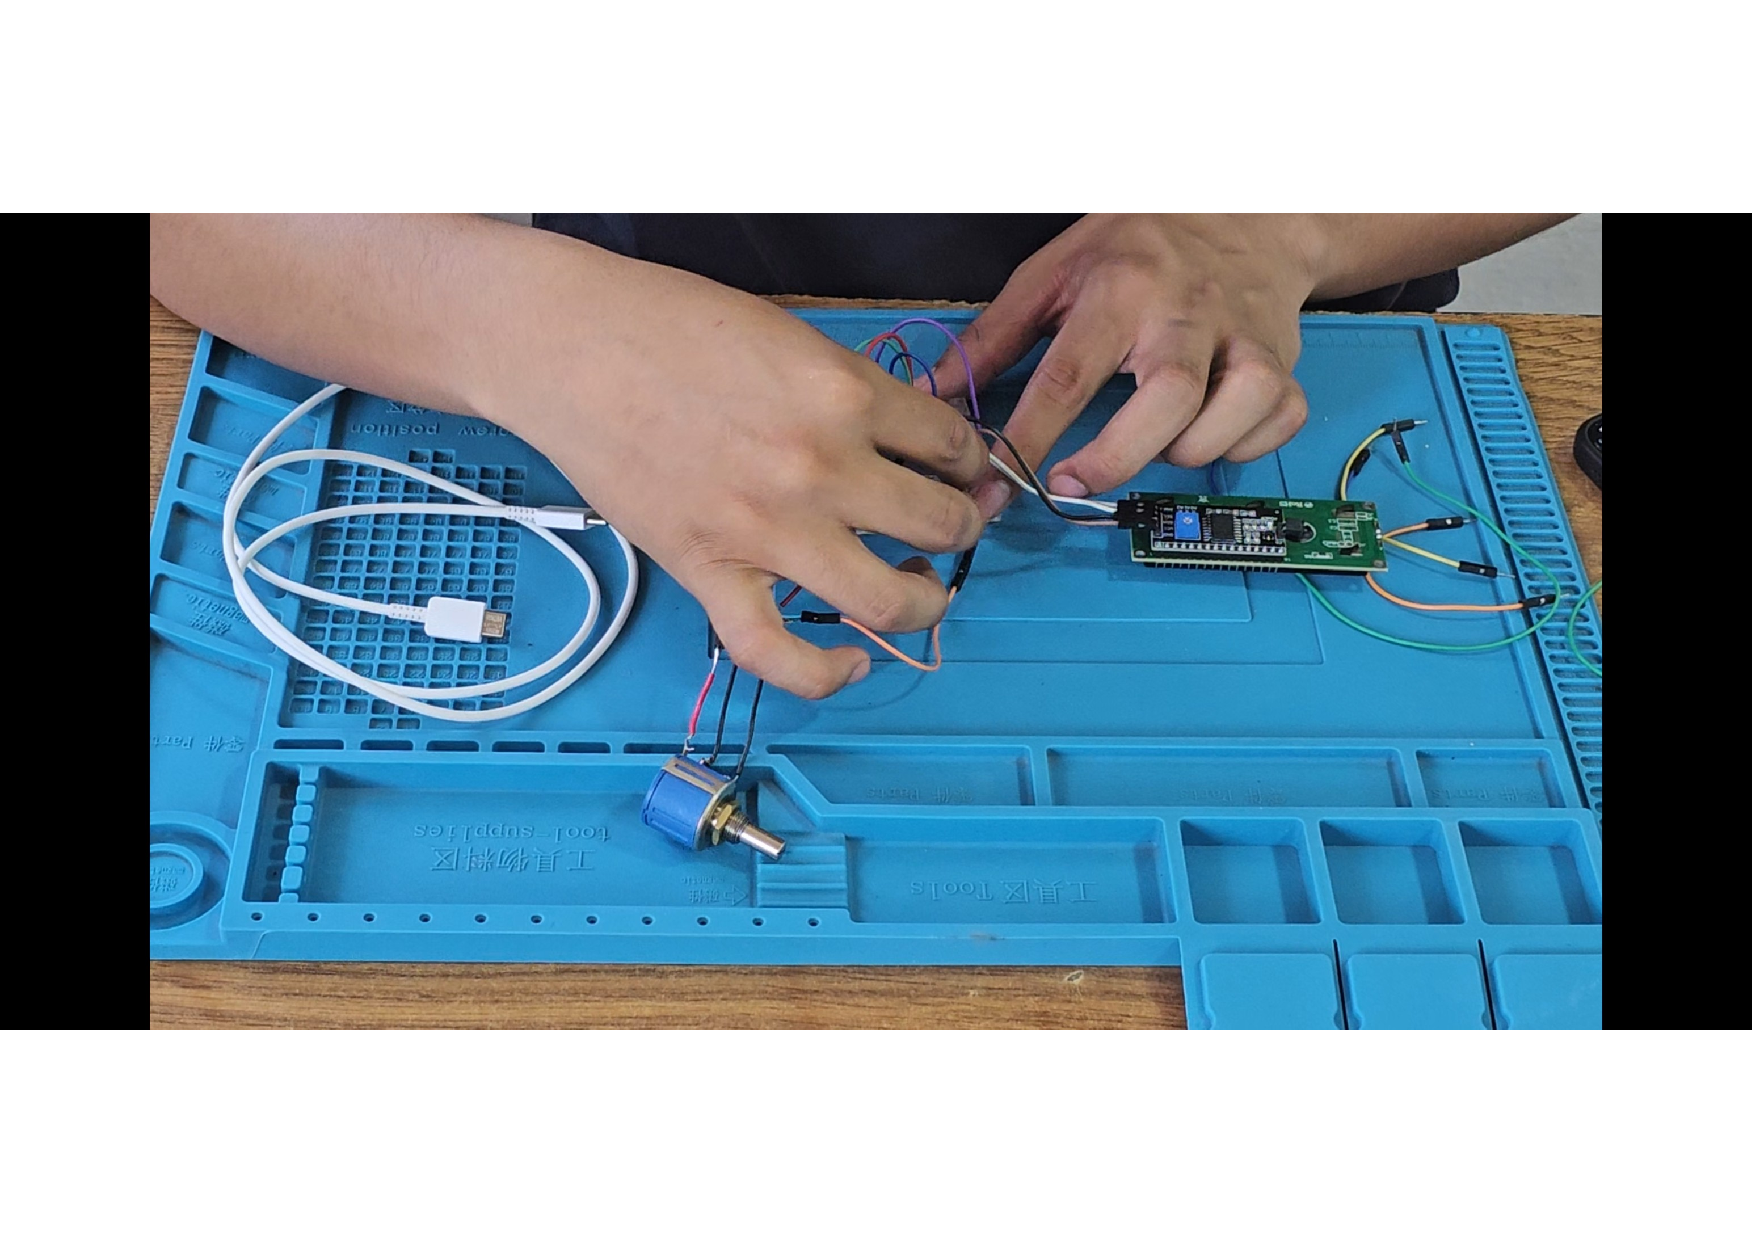
\includegraphics[trim = {7mm 1mm 1mm 1mm},clip,scale=0.25]{22/Img/e8.pdf}
        \caption{Colocación de la LCD}
        \label{fig:evi3}
    \end{figure}
    
    
    \begin{figure}[H]
        \centering
        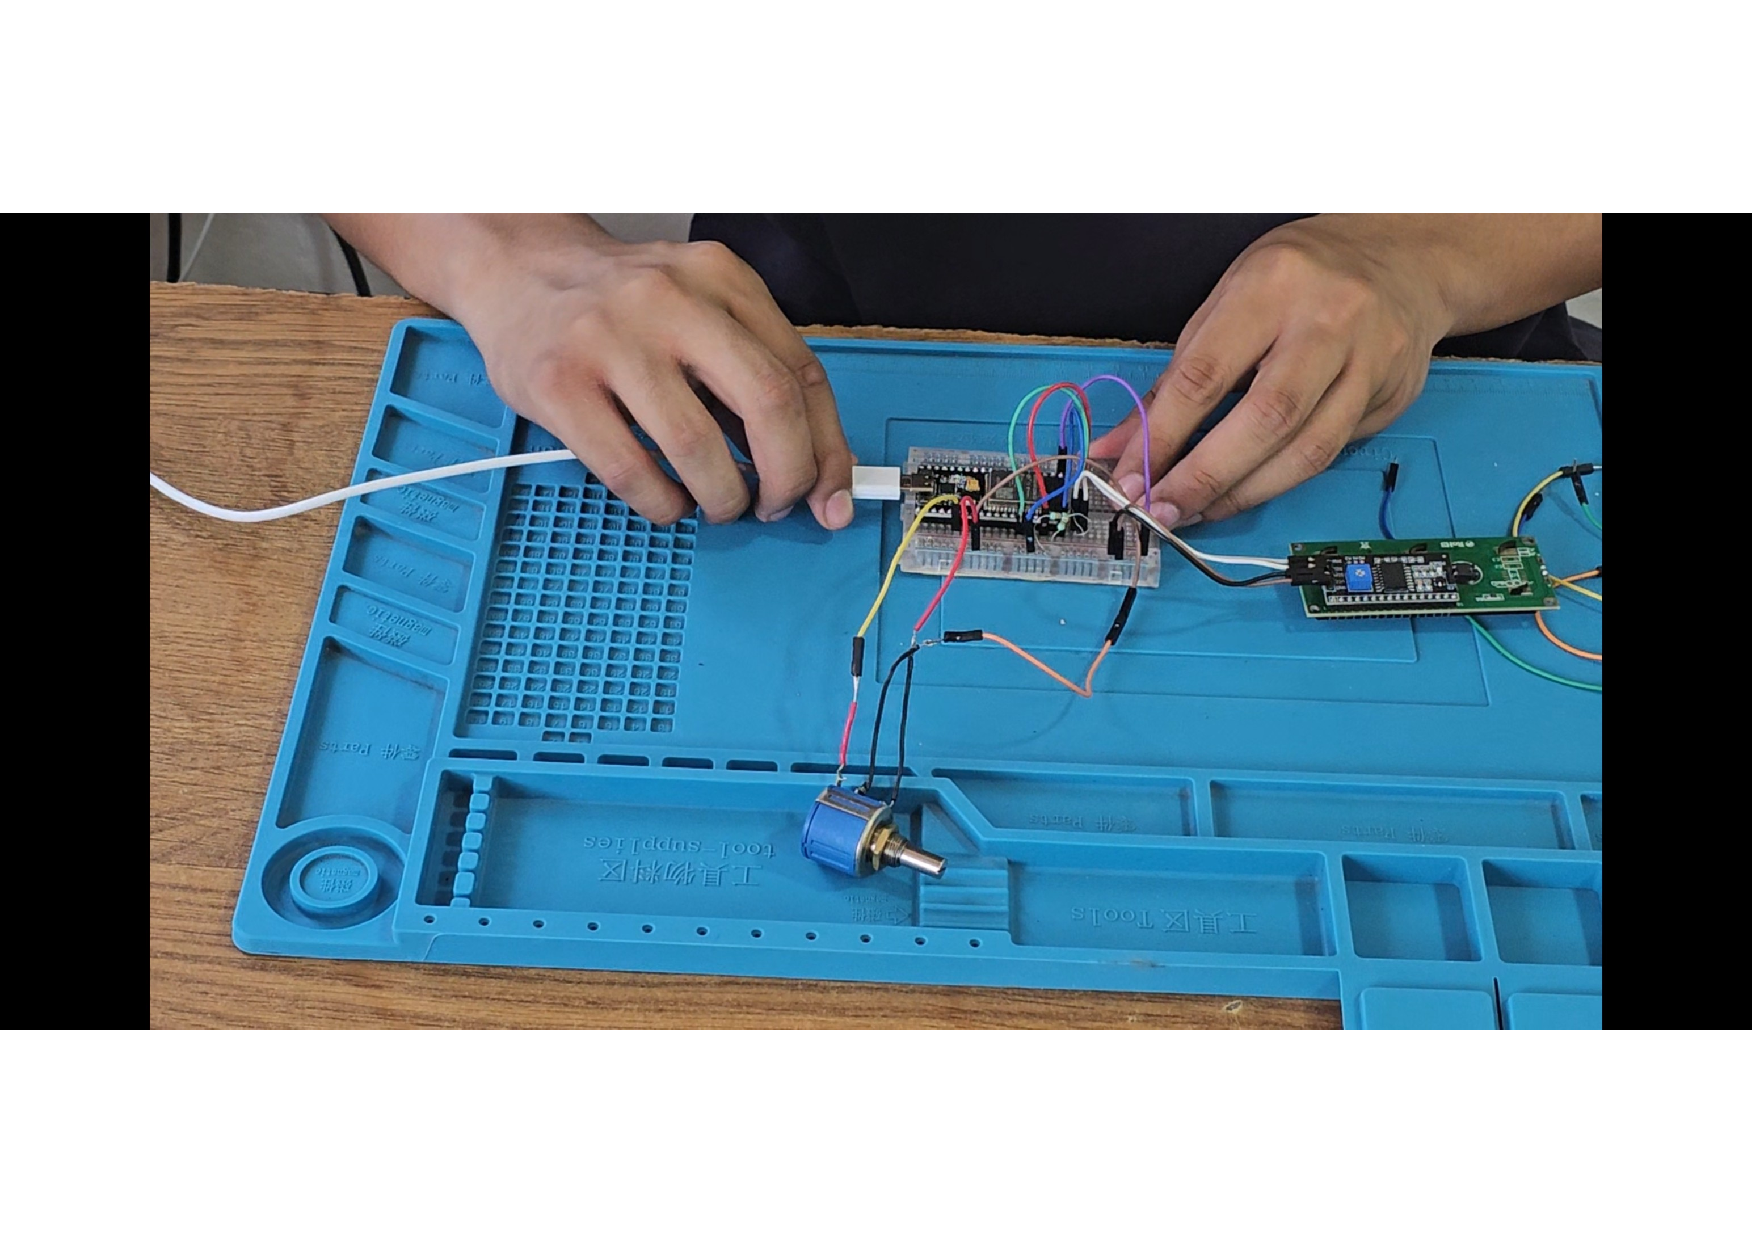
\includegraphics[trim = {7mm 1mm 1mm 1mm},clip,scale=0.25]{22/Img/e10.pdf}
        \caption{Conexión al cable C}
        \label{fig:evi4}
    \end{figure}
    
    
    \begin{figure}[H]
        \centering
        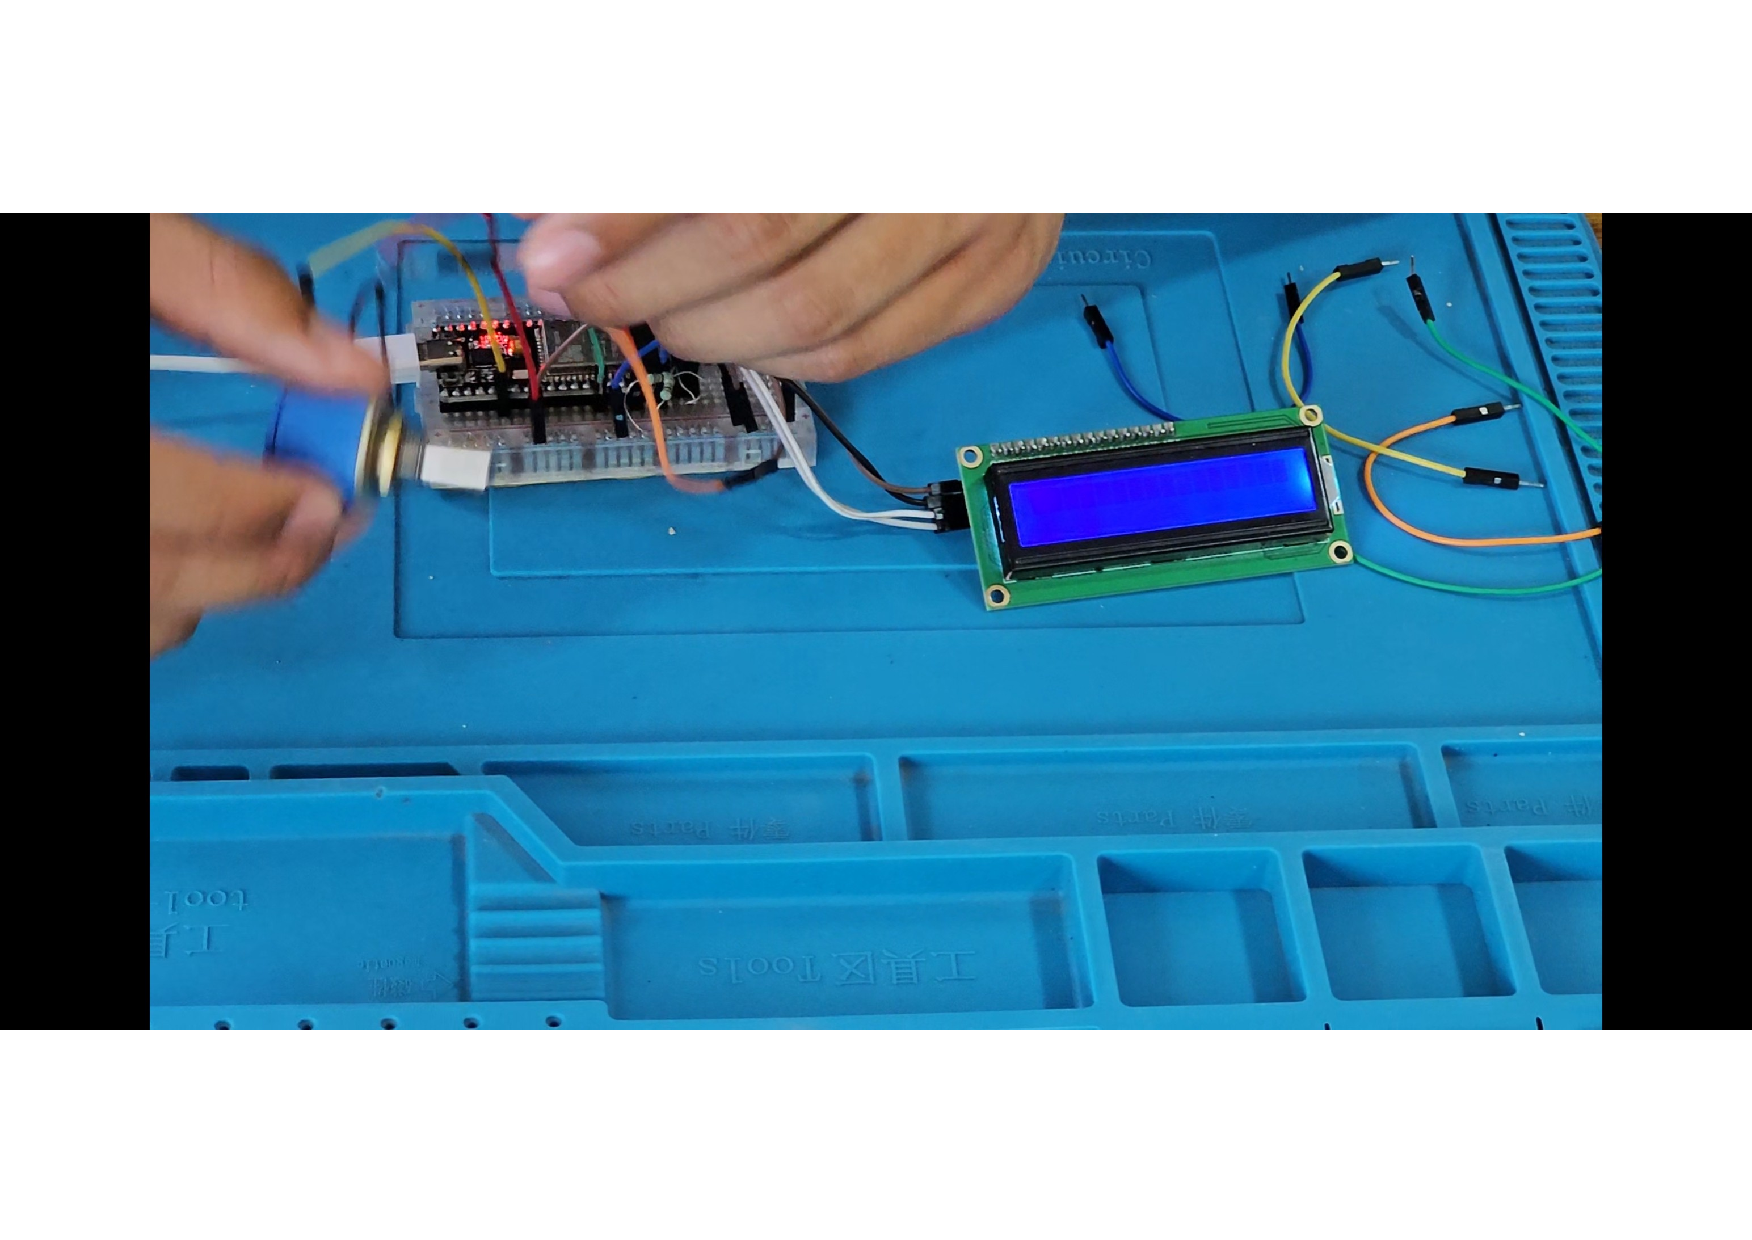
\includegraphics[trim = {7mm 1mm 1mm 1mm},clip,scale=0.25]{22/Img/e12.pdf}
        \caption{Proceso de encendido de la LCD}
        \label{fig:evi5}
    \end{figure}
    
    
    \begin{figure}[H]
        \centering
        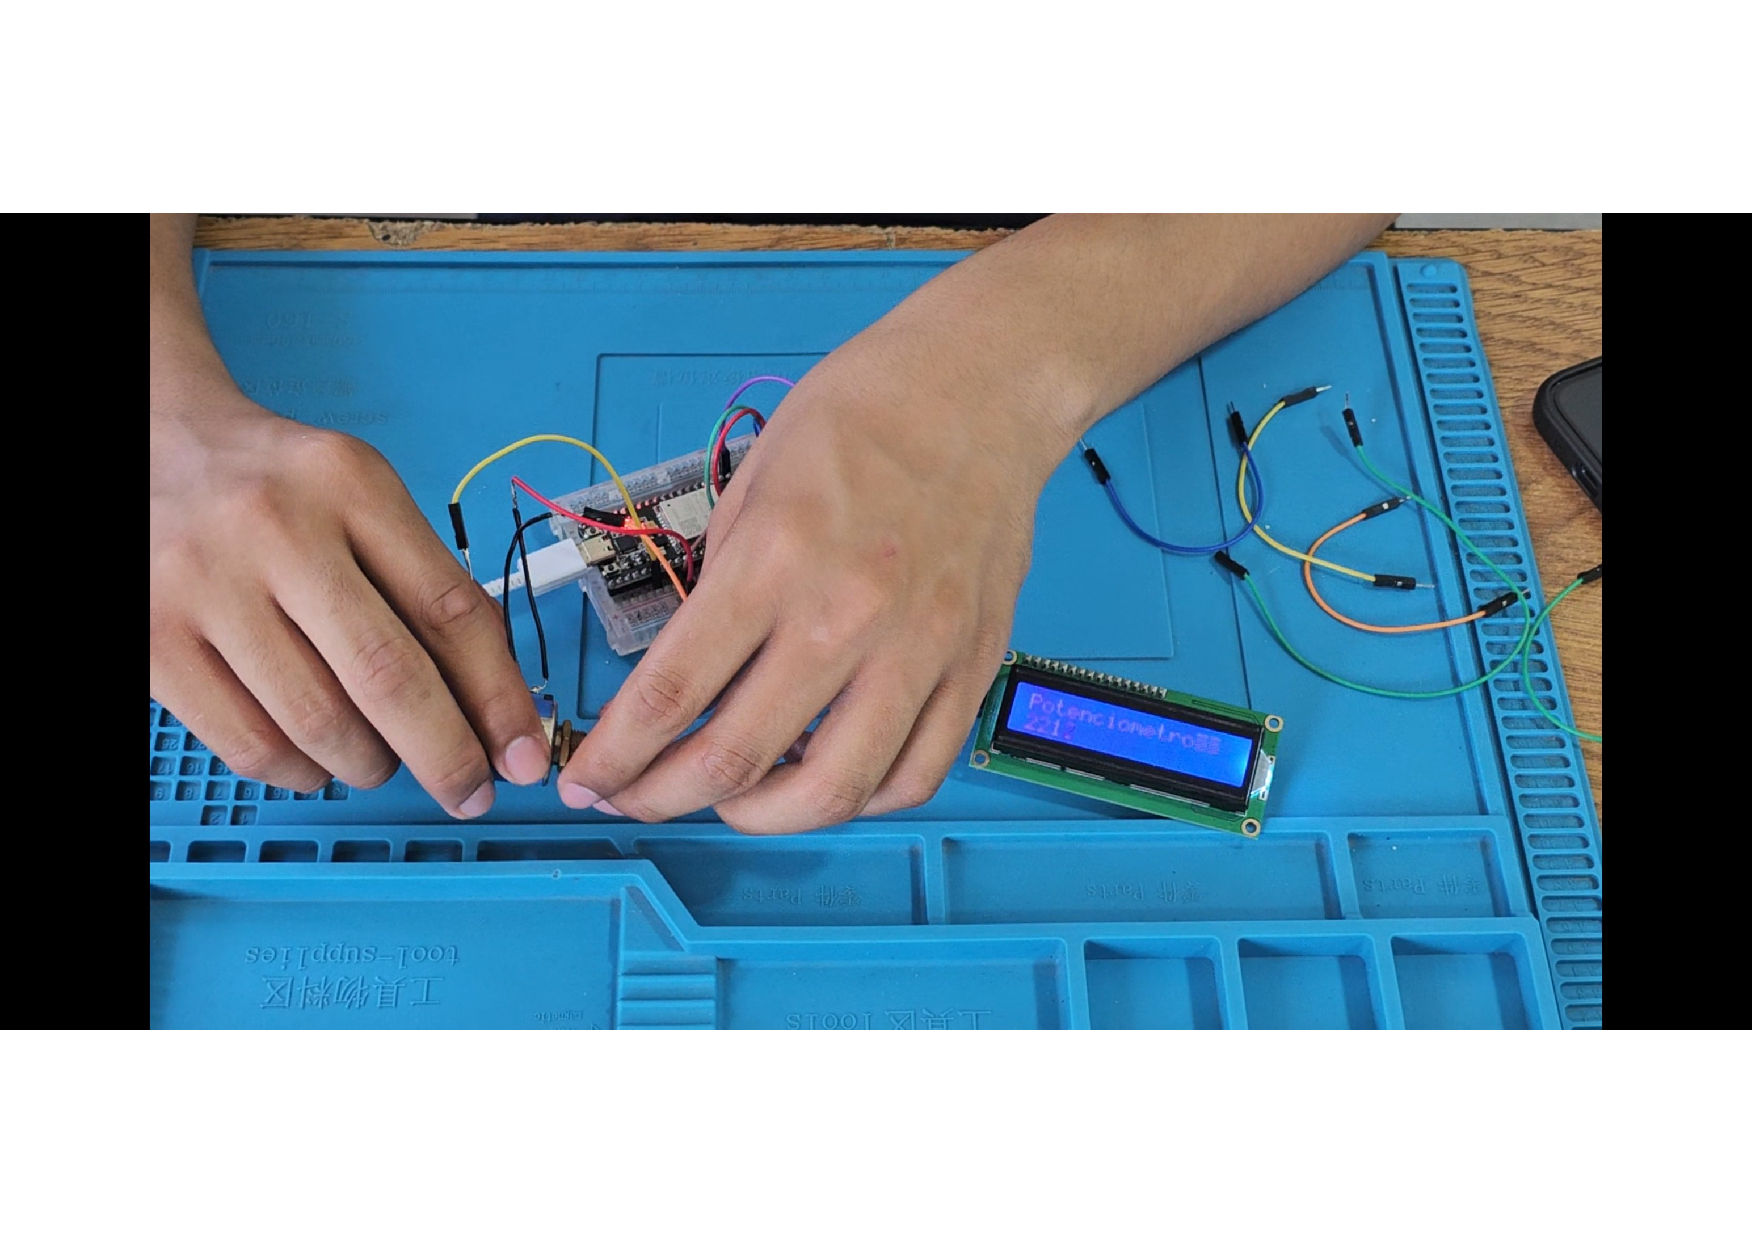
\includegraphics[trim = {7mm 1mm 1mm 1mm},clip,scale=0.25]{22/Img/e15.pdf}
        \caption{Interacción con el potenciometro}
        \label{fig:evi6}
    \end{figure}
    
    
    \begin{figure}[H]
        \centering
        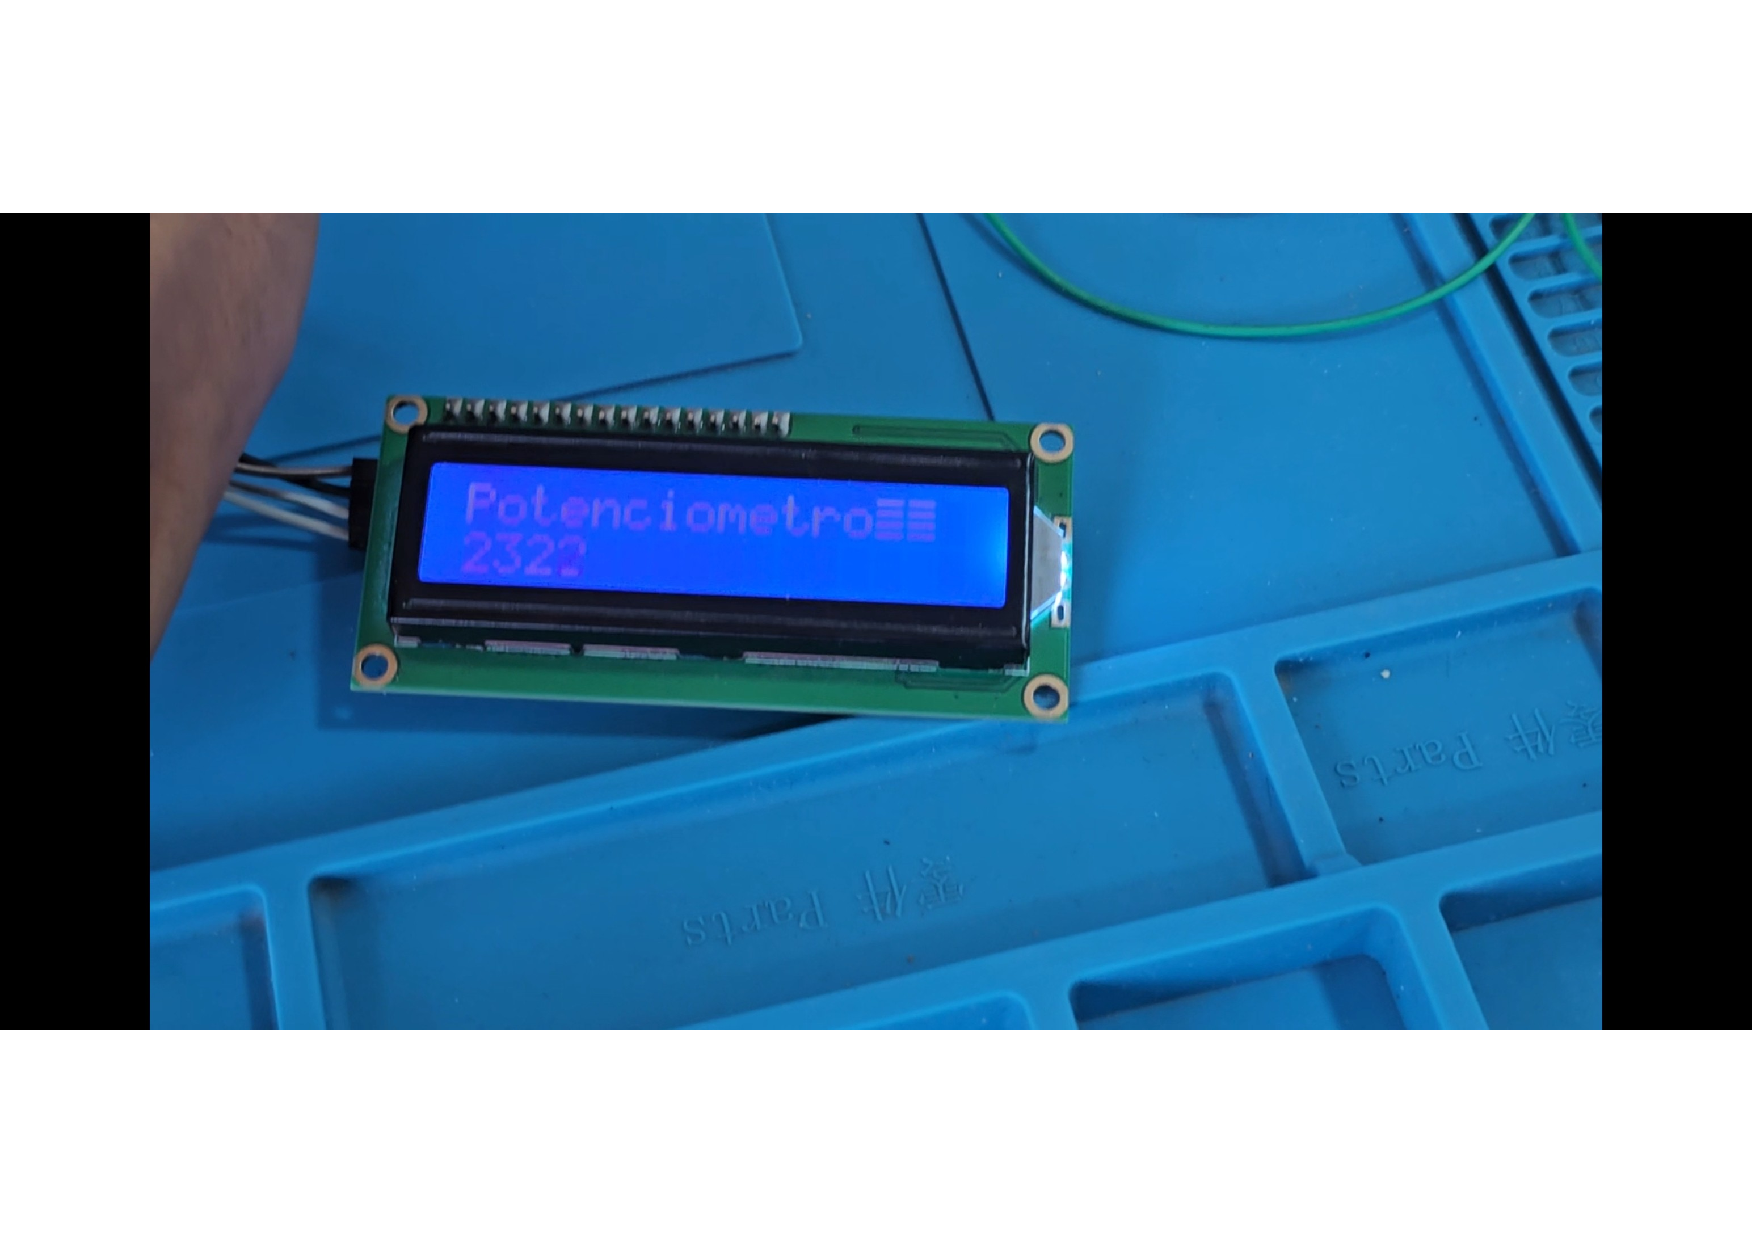
\includegraphics[trim = {7mm 1mm 1mm 1mm},clip,scale=0.25]{22/Img/e17.pdf}
        \caption{Encuadre de la LCD}
        \label{fig:evi7}
    \end{figure}
    
    
    \begin{figure}[H]
        \centering
        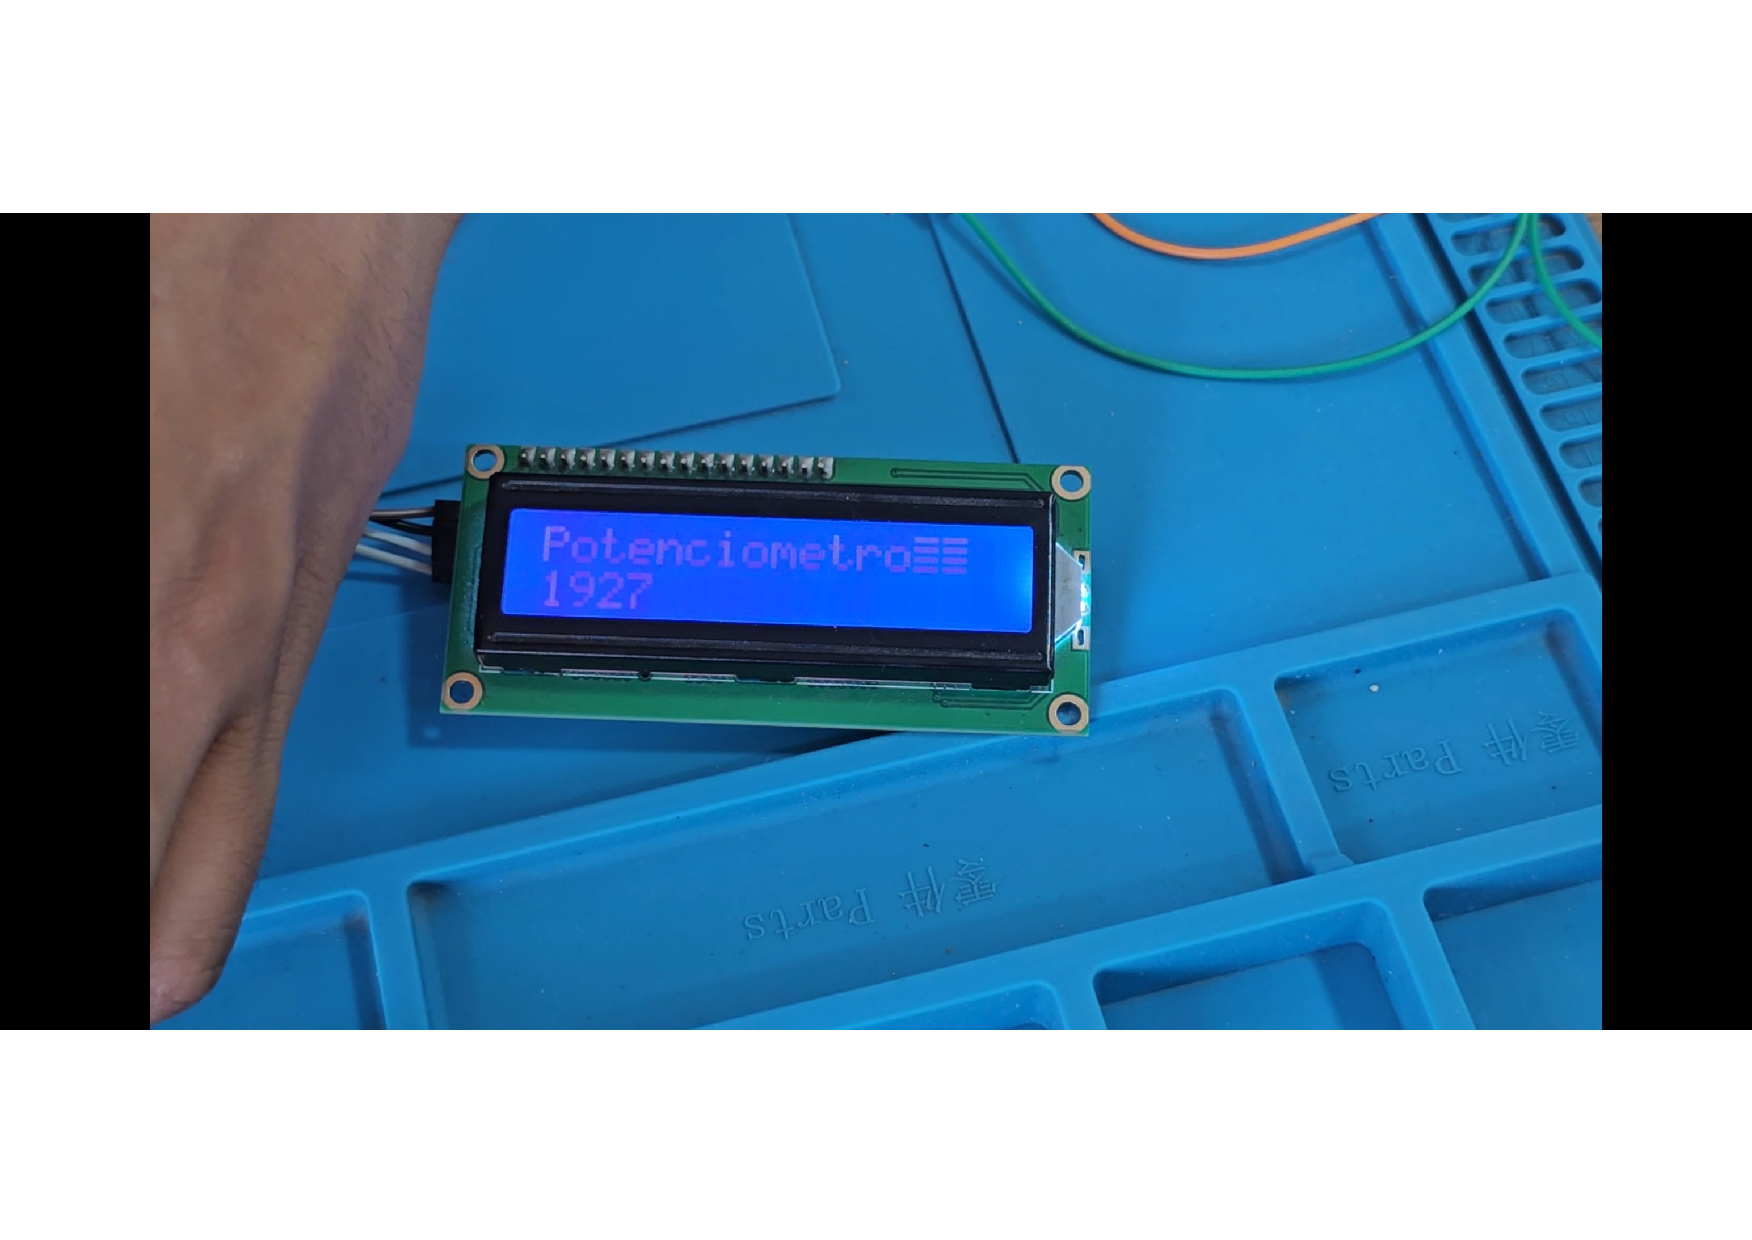
\includegraphics[trim = {7mm 1mm 1mm 1mm},clip,scale=0.25]{22/Img/e20.pdf}
        \caption{Cambio de valor}
        \label{fig:evi8}
    \end{figure}
    
    
    \subsection{Autores y Afiliaciones}
    
    \subsection{Tablas y Figuras}
    
    \section{Conclusiones}
    
    
    
    \section{Agradecimientos}
    
    
    \section{Referencias}
    
    
    
    
    % \newpage
    % \bibliographystyle{ieeetr}
    % \bibliography{22/referencias}
    % 
    % 
    %%%%%%%%%%%%%%%%%%%%%%%%%%%%%%%%%%
    \appendix
    %%%%%%%%%%%%%%%%%%%%%%%%%%%%%%%%%%
    % 
    \centering{\section[\appendixautorefname{}]{Apéndice Instructivo}}\label{Figura:instructivo}
    \includepdf[pages=3-5 ]{22/Img/instructivoMateriales.pdf}
    %%%%%%%%%%%%%%%%%%%%%%%%%%%%%%%%%%%%%%%%
    % 
    \centering{\section[\appendixautorefname{}]{Apéndice Materiales}}\label{Figura:Materiales}
    \includepdf[pages=6-7,]{22/Img/instructivoMateriales.pdf}
    % 
    %%%%%%%%%%%%%%%%%%%%%%%%%%%%%%%%%%%%%%%%
    \centering{\section[\appendixautorefname{}]{Apéndice de Formato}}\label{Figura:Hoja de datos}
    \includepdf[pages=-,]{22/Img/formato.pdf}
    
    
    \newpage
    \bibliographystyle{ieeetr}
    \bibliography{22/referencias}